\documentclass[11pt]{article}

% ---------- Fonts & micro-typography ----------
\usepackage[T1]{fontenc}
\usepackage{newtxtext}            % Times-like text
\usepackage{microtype}
\usepackage[ruled,vlined]{algorithm2e}

% ---------- Page layout ----------
\usepackage[margin=1in]{geometry} % 1in margins; adjust if needed
\setlength{\headheight}{14pt}     % satisfy fancyhdr requirement
\usepackage{setspace}
\setstretch{1.05} % subtle tightening

% ---------- Math & theorems ----------
\usepackage{amsmath,amssymb,amsthm,mathtools,bm}
\usepackage{newtxmath}            % Times-like math (must load AFTER amsthm/amssymb)
\numberwithin{equation}{section}
\theoremstyle{plain}
\newtheorem{theorem}{Theorem}[section]
\newtheorem{lemma}[theorem]{Lemma}
\newtheorem{corollary}[theorem]{Corollary}
\newtheorem{proposition}[theorem]{Proposition}
\theoremstyle{definition}
\newtheorem{definition}[theorem]{Definition}
\theoremstyle{remark}
\newtheorem{remark}[theorem]{Remark}
\newtheorem{thm}[theorem]{Theorem}
\newtheorem{cor}[theorem]{Corollary}

% Common operators (optional but tidy)
\DeclareMathOperator{\E}{\mathbb{E}}
\DeclareMathOperator{\Var}{\mathbb{V}\mathrm{ar}}
\DeclareMathOperator{\Tr}{Tr}

% ---------- Figures, tables, lists ----------
\usepackage{graphicx}
\usepackage{subcaption}
\usepackage{booktabs}
\usepackage{caption}
\captionsetup{labelfont=bf}
\usepackage{enumitem}
\setlist{itemsep=2pt,topsep=4pt}

% ---------- Cross-references ----------
\usepackage{hyperref}
\usepackage[nameinlink,capitalise,noabbrev]{cleveref}

% ---------- Bibliography (biblatex) ----------
\usepackage[backend=biber,
  style=numeric,sorting=nyt,maxnames=10,giveninits=true,
  doi=true,url=false,eprint=false
]{biblatex}
\addbibresource{sample.bib}
\addbibresource{biblio.bib}

% ---------- Authorship block ----------
\usepackage{authblk}
\renewcommand\Authfont{\large}
\renewcommand\Affilfont{\normalsize\normalfont}
\setlength{\affilsep}{0.5em}
\renewcommand\Authands{ and }

% ---------- Hyphenation ----------
\hyphenation{de-si-de-rium}

% ---------- Page styles (journal-like) ----------
% --- Header (preprint-friendly journal style) ---
\usepackage{fancyhdr}
\usepackage{etoolbox} % for \ifstrempty
% \usepackage[hidelinks]{hyperref} % (make sure hyperref is loaded somewhere)

% Leave these empty for now; fill them later if you get a venue/DOI.
\newcommand{\journalname}{}     % e.g., "Journal of ..."
\newcommand{\paperrange}{}      % e.g., "1--17"
\newcommand{\paperdoi}{}        % e.g., "https://doi.org/...."
\newcommand{\articletype}{Preprint}
\newcommand{\versiondate}{\today}

% Running heads (edit these two lines)
\newcommand{\runningtitle}{RHTDistributedRegression}
\newcommand{\runningauthor}{Yang}

% Header texts (auto-fallbacks)
\newcommand{\leftheader}{%
  \ifstrempty{\journalname}{\articletype}{\journalname}%
}
\newcommand{\rightheader}{%
  \ifstrempty{\paperrange}{%
    \ifstrempty{\paperdoi}{Version:\,\versiondate}{DOI:\,\href{\paperdoi}{\paperdoi}}%
  }{%
    \paperrange%
    \ifstrempty{\paperdoi}{}{ \quad DOI:\,\href{\paperdoi}{\paperdoi}}%
  }%
}

\fancypagestyle{firstpage}{%
  \fancyhf{}
  \fancyhead[L]{\footnotesize\textsc{\leftheader}}
  \fancyhead[R]{\footnotesize \rightheader}
  \renewcommand{\headrulewidth}{0pt}
}
\pagestyle{fancy}
\fancyhf{}
\fancyhead[R]{\thepage}
\fancyhead[L]{\small\textsc{\runningtitle}}
\renewcommand{\headrulewidth}{0.4pt}
% ---------- Title helpers ----------
\newcommand{\keywords}[1]{\noindent\textbf{Keywords}: #1}





% ----- title & authors (ARTICLE + AUTHBLK) -----
\title{The Merits of Randomized Hadamard Transform in Distributed Regression via Partitioned Machines}
\author{Yishu Yang}
\affil{Center for Data Science, New York University, New York. \texttt{fergie.yang@nyu.edu}}
\date{} % empty (sample had no date)
\newcommand{\dedicated}[1]{\begin{center}\emph{#1}\end{center}}
\begin{document}
\thispagestyle{firstpage}
\maketitle
\dedicated{The development of this work is supervised by Prof. Zhixiang Zhang at University of Macau, zhixzhang@um.edu.mo}
\keywords{Distributed Sketching, Ordinary Least Squares (OLS), Randomized Hadamard Transform (RHT), Partitioned Machines, Relative Efficiency, Gaussian Mixture Model (GMM)}
\begin{abstract}
In the time of large-scale data analysis, distributed sketching has emerged as a pivotal technique for efficiently training linear regression models on massive datasets. This paper examines the relative efficiency of distributed Ordinary Least Squares (OLS) estimation using partitioned machines, with a focus on the impact of various sampling methods. We identify a specific scenario where uniform sampling in distributed sketching leads to a significant decrease in relative efficiency, particularly when the data matrix follows a Gaussian Mixture Model (GMM) characterized by biased variance across different data rows. Our primary contribution lies in demonstrating that the application of the Randomized Hadamard Transform (RHT) before partitioning 
can substantially enhance the relative efficiency of OLS estimation. By flattening the variance of the local Gram matrices across machines, RHT enables efficient equal-weighted averaging of local OLS estimators, avoiding the need for complex weight adjustments. We rigorously prove that under the condition of sublinear growth of the number of features $p$ concerning the number of samples $n$,
 specifically when $\ln n = o(p(n))$ and $p(n)\ln p(n) = o(n)$, the relative efficiency of OLS estimation with equal-weighted partitions after RHT asymptotically approaches the ideal value of 1 as $n$ tends to infinity. 
 This implies that the difference between the trace of the inverse of the local Gram matrix and the trace of the inverse of the scaled global Gram matrix converges to zero at a specific rate. Experimental results corroborate our theoretical findings, highlighting the merits of RHT in achieving the relative efficiency that approaches 1 in distributed OLS regression under the considered data distribution and dimensionality conditions.
\end{abstract}

% Ensure all metadata is properly defined above this line.





\section{Introduction}
In the era of big-scale data analysis, distributed sketching in machine learning has been a common tool for efficiently training large datasets for most linear regression tasks. This means we would partition our full datasets into $K$ blocks and then do the regression on each block separately, which is followed by an averaged process of all the learned local parameters to get an overall parameter.
This has been studied much by researchers in the field of distributed machine learning, however, many researchers focus on the optimized absolute sketching errors or proportions of biases in distributed sketching (Wang, 2018\cite{wang2018sketchedridgeregressionoptimization}) or focus on the accurate expectation of approximation error for the OLS (ordinary least square) estimation (Derezinski, 2023\cite{dereziński2023algorithmicgaussianizationsketchingconverting}). Not much work has been done to compare the relative efficiency of different sampling methods in distributed sketching, like Subsampled Randomized Hadamard Transform Sampling (SRHT) or Leverage-based Sampling (LBS).
However, it is good to see that Dobriban and Liu\cite{dobriban2019asymptoticssketchingsquaresregression} have discussed many results of distributed sketching in OLS estimation via all kinds of efficiencies, which I think would be a further study regarding our research here.

In this article, our main research contribution is to identify the specific distribution of the data matrix $\mathbf{X}$ where the relative efficiency of OLS estimation, i.e., the error ratio of global OLS estimator to distributed OLS estimator by averaging local OLS estimators, would decrease drastically when the sampling method is just the equally partitioned uniform sampling from the "$Section 3.2$ Finite sample results" of the paper by Dobriban and Sheng\cite{dobriban2022distributedlinearregressionaveraging}.
And we contribute to show that the Randomized Hadamard Transform (RHT) here could improve the relative efficiency of OLS estimation by flattening the variance of the local gram matrix for each machine with equal weight for averaging, thus helping us save the time for adjusting th weight accordingly from the result of \ref{eq:2.7}. Finally, our most important contribution is to rigorouly proving that the relative efficiency of OLS estimation with equal-weighted partitions after Randomized Hadamard Transform (RHT) could achieve the dream efficiency of 1 when the number of rows $n$ tends to infinity and the number of columns $p$ also tends to infinity but is the sublinear growth of $n$ larger than the logarithmatic growth of $n$.\ref{corollary:main}
We could also intepretate this idea differently, that is the difference of $\operatorname{tr}[(\tilde{\mathbf{X}}_i^{\top}\tilde{\mathbf{X}}_i)^{-1}]$ and $\operatorname{tr}[(\frac{1}{K}\tilde{\mathbf{X}}^{\top}\tilde{\mathbf{X}})^{-1}]$ converges to $0$ at the rate of $\mathcal{O}(\sqrt{p^{3}\frac{\log n}{n^{3}}})$\ref{eq:4.5} as $n$ tends to be approaching infinity for $p$ satisfying sublinear growth of $n$ larger than logarithmatic growth of $n$, meaning that the local gram matrix after Randomized Hadamard Transform (RHT) is well stablized.

In short, we skip the dirty work of adjusting the weight for each local OLS estimator and just take the average of all local OLS estimators with equal weight $\frac{1}{K}$ for $K$ machines by utilizing the Randomized Hadamard Transform (RHT) to flatten the variance of the local gram matrix for each machine.

Our main intuition of randomized hadamard transfrom {RHT} is from the paper of Tropp\cite{tropp2011improvedanalysissubsampledrandomized} and the paper of Cherapanamjeri\cite{cherapanamjeri2022uniformapproximationsrandomizedhadamard}. And we utilize many probability inequalities from the book of Vershynin\cite{vershynin2018high}, the papers of Tropp\cite{tropp2011improvedanalysissubsampledrandomized} and \cite{Tropp_2011}, mainly the Bernstein Inequality of sub-exponential tail bounds and Matrix Chernoff Inequality to prove the result of Corollary~\ref{corollary:main}.
\section{Main Result: RHT with equal partitions for regression}
Our main contribution here is that under the research target of Dobriban and Sheng \cite{dobriban2022distributedlinearregressionaveraging} for the finite sampling results of relative efficiency of global OLS estimator to distributed OLS estimator, we focus on
what kinds of distribution would let uniform sampling partitions decrease the relative efficiency drastically and RHT could help resolve it. (two methods in Remark~\ref{remark:sampling})

The idea of normalized Hadamard matrix is as follows:
A square matrix \( \mathbf{H} \) of dimension \( n \times n \), possibly complex, is a Hadamard matrix if \( \mathbf{H} / \sqrt{n} \) is orthogonal and \( |\mathbf{H}_{ij}| = 1 \) for all \( i, j = 1, \ldots, n \). An example is the Walsh-Hadamard matrix, defined recursively as:
\[
\mathbf{H}_n = \begin{pmatrix} \mathbf{H}_{n/2} & \mathbf{H}_{n/2} \\ \mathbf{H}_{n/2} & -\mathbf{H}_{n/2} \end{pmatrix},
\]
where \( \mathbf{H}_{n/2} \) is the Walsh-Hadamard matrix of order \( n/2 \) and \( \mathbf{H}_1 = 1 \). The Hadamard matrix is orthogonal, meaning \( \mathbf{H}_n \mathbf{H}_n^T = n\mathbf{I}_n \), where \( \mathbf{I}_n \) is the identity matrix of order \( n \).

We chose a distribution called Gaussian Mixture Model (GMM) distribution (defined in Definition~\ref{def:gmm}), and found that uniform sampling would perform bad in this case in terms of the finite sample results of relative efficiency of OLS estimation between global and distributed estimators proposed by Dobriban and Sheng \cite{dobriban2022distributedlinearregressionaveraging} (Lemma~\ref{lem:finiteresults}) for equal-weight averaging.

Then our major contribution is that we show RHT could flatten the variance so that we could achieve a perfect relative efficiency $\mathbb{E}(\mathbf{I}_p,\tilde{\mathbf{X}}_1,...,\tilde{\mathbf{X}}_K) = 1$ when $n$ tends to infinity. (See Main Result: Corollary~\ref{corollary:main})

Here the setting is the most general linear regression on the given matrix $\mathbf{X}$ and $\mathbf{Y}$ where the true relationship is $\mathbf{Y} = \mathbf{X}\beta + \epsilon$, $\epsilon\sim\mathcal N(0,\mathbf{I}_n)$, and we do ordinary least square (OLS) regression on the given matrix $\mathbf{X}$ and $\mathbf{Y}$.
Then we could measure the quality of linear regression by doing the expected mean square error (MSE) on the given matrix $\mathbf{X}$ and $\mathbf{Y}$.

In the standard linear regression model $\mathbf{Y} = \mathbf{X}\beta + \epsilon$, $\beta \in \mathbb{R}^p$ represents the true, unknown parameter vector we aim to estimate. The matrix $\mathbf{X} \in \mathbb{R}^{n \times p}$ contains the predictor variables (data), $\mathbf{Y} \in \mathbb{R}^n$ contains the response variables, and $\epsilon \in \mathbb{R}^n$ represents the noise term, typically assumed to have zero mean and identity covariance matrix ($\epsilon \sim \mathcal{N}(0, \sigma^2 \mathbf{I}_n)$, often with $\sigma^2=1$ for simplicity in theoretical analysis).

The Ordinary Least Squares (OLS) estimator, denoted by $\hat{\beta}$, provides an estimate of $\beta$ based on the observed data $(\mathbf{X}, \mathbf{Y})$. It is calculated by minimizing the sum of squared differences between the observed responses $\mathbf{Y}$ and the predicted responses $\mathbf{X}b$:
\[
\hat{\beta} = \arg\min_{b \in \mathbb{R}^p} ||\mathbf{Y} - \mathbf{X}b||_2^2
\]
Assuming $\mathbf{X}$ has full column rank (i.e., $\mathbf{X}^{\top}\mathbf{X}$ is invertible), the unique solution is given by the normal equations:
\[
\hat{\beta} = (\mathbf{X}^{\top}\mathbf{X})^{-1}\mathbf{X}^{\top}\mathbf{Y}
\]
The quality of this estimator is often assessed by its Mean Squared Error (MSE), which measures the expected squared Euclidean distance between the estimator $\hat{\beta}$ and the true parameter $\beta$. For a fixed design matrix $\mathbf{X}$,

we denote as $M(\hat{\beta}) = \mathbb{E}||\beta - \hat{\beta}||^2$
where $\hat{\beta}$ is the OLS estimator of $\beta$.
Since the matrix $\mathbf{X}$ and $\mathbf{Y}$ could have infinity many number of rows, i.e., $n$ could tend to infinity, OLS estimation would be of much computational burden with exponential training time.

So the general ideas to do the regression here to prevent computational burden is by distributed sketching, that we allcoate sub training sets into many local machines and then do training on each sub machines as well as an aggregated averaging estimators. Here our main part is using partitioned machines to do the regression.

The averaging estimator is given by $\hat{\beta}_{\text{\footnotesize \textit{dist}}} = \sum_{i=1}^K w_i \hat{\beta}_i$, where the ratio associated to it is $w_i$ for each machine $i = 1,2,\ldots,K$.
We denote as $M(\hat{\beta}_{\text{\footnotesize \textit{dist}}}) = \mathbb{E}||\beta - \hat{\beta}_{\text{\footnotesize \textit{dist}}}||^2$
where $\hat{\beta}_{\text{\footnotesize \textit{dist}}}$ is the distributed estimator of $\beta$.
Thus the relative efficiency is defined by Lemma~\ref{lem:finiteresults} as $E(\mathbf{X}_1,\dots,\mathbf{X}_K) = \frac{M(\hat{\beta})}{M(\hat{\beta}_{\text{\footnotesize \textit{dist}}})}$.

Firstly, we will talk about why we choose to uniformly partition these machines and what is the case if we don't do RHT here, and what kind of $E(\mathbf{I}_p,\mathbf{X}_1,...,\mathbf{X}_K)$ we could achieve, then we will discuss that if we use RHT before doing uniform sampling in partitions, we should not adjust $w_i$ and just take average by $\frac{1}{K}$. (Lemma~\ref{lemma:expectation})

Note: this paper discuss the situation of infinitly high dimention, where $n$ could be as large as infinity and $p$ satisfies being the sublinear growth of $n$ that is larger than logarithmatic growth of $n$, which means $p$ could also approaches $\infty$ being a smaller level of infinity than $n$.
\begin{remark}[Growth Conditions for Parameter $p(n)$]
\label{remark:sublinear}
In our asymptotic analysis, we require the parameter $p(n)$, a function $p: \mathbb{N} \to \mathbb{R}^+$, to adhere to a specific growth regime ensuring desirable convergence properties for probability bounds. We term this \emph{controlled intermediate growth}, defined by the following conditions as $n \to \infty$:
\begin{itemize}
    \item[(C1)] $p(n)$ is superlogarithmic with respect to $n$: $\ln n = o(p(n))$, meaning $\lim_{n \to \infty} \frac{\ln n}{p(n)} = 0$.
    \item[(C2)] $p(n)\ln p(n)$ is sublinear with respect to $n$: $p(n)\ln p(n) = o(n)$, meaning $\lim_{n \to \infty} \frac{p(n)\ln p(n)}{n} = 0$.
\end{itemize}
Condition (C1) ensures $p(n)$ dominates logarithmic factors of $n$. Condition (C2) ensures $p(n)$ does not grow too rapidly, specifically, slower than $n/\ln p(n)$. Standard examples of $p(n)$ satisfying (C1) and (C2) include $p(n) = n^a$ for any $a \in (0,1)$, $p(n) = (\ln n)^k$ for $k > 1$, and $p(n) = n/(\ln n)^k$ for $k > 1$.
\end{remark}

Now this is our main result of this paper, that is the relative efficiency of OLS estimation with equal-weighted partitions after RHT could achieve the dream efficiency of 1 when $n$ tends to infinity and $p$ satisfies Remark\ref{remark:sublinear}.
\begin{corollary}
  \label{corollary:main}
  Let $\mathbf{X}\in\mathbb{R}^{n\times p}$ be the assumed full rank matrix such that each row of $\mathbf{X}$ is i.i.d.\ sampled from the proposed Gaussian Mixture Model (GMM) distribution (Definition~\ref{def:gmm}) where there are totally $n$ rows and number of features $p$ satisfies Remark\ref{remark:sublinear}.

  $\mathbf{\tilde{X}} = \mathbf{H}_n\mathbf{D}\mathbf{X}$, where $\mathbf{H}_n$ is the normalized Hadamard matrix of order $n$, and $\mathbf{D}$ is the Rademacher matrix of order $n$ with diagnoal entries $d_1, d_2, \ldots, d_n$ to be 1 or -1 with equal probability.

  And $\mathbf{\tilde{X}}_{1}, \mathbf{\tilde{X}}_{2}, \ldots, \mathbf{\tilde{X}}_{K}$ are the partitioned machine submatrices after being Randomzied Hadamard Transformed (RHT) from Remark~\ref{remark:sampling}.

  Then, based on the \ref{eq:2.4} result of Lemma~\ref{lem:finiteresults}, we have the following corollary:
  \[
    \lim_{n\to\infty}\mathbb{E}(\mathbf{\tilde{X}}_1,\ldots,\mathbf{\tilde{X}}_K) = 1
  \]
  as long as the condition of Remark~\ref{remark:sublinear} is satisfied.
\end{corollary}
\subsection{Our focus on proving better relative efficiency[main focus]}
We first give the finite sample results of Dobriban and Sheng \cite{dobriban2022distributedlinearregressionaveraging} from their paper's section $\S$3.2 as our lemma \ref{lem:finiteresults} here.

\begin{lemma}[Relative Efficiency of distributed linear regression in partitions]
  \label{lem:finiteresults}

    Let \(\mathbf{X}\in\mathbb{R}^{n\times p}\) be the assumed full rank matrix and $M(\hat{\beta}) = \mathbb{E}||\beta - \hat{\beta}||^2$ be the expected Mean Square Error of OLS estimation.
    
    Here the relative efficiency is defined as
    \[
    E(\mathbf{X}_1,\dots,\mathbf{X}_K) = \frac{M(\hat{\beta})}{M(\hat{\beta}_{\text{\footnotesize \textit{dist}}})},\tag{2.1} \label{eq:2.1}
    \]
    where \({\mathbf{X}}_{1}, \ldots, {\mathbf{X}}_{K}\) are the partitioned submatrices as described in Remark~\ref{remark:sampling}.

    We have the following results of Expected MSE for global OLS linear regression, partitioned OLS linear regression and Relative Efficiency:
    \begin{enumerate}
    \item The mean–squared error of the global OLS estimator is
          \[
            M(\hat\beta)=\operatorname{tr}\!\bigl[(\mathbf{X}^{\top}\mathbf{X})^{-1}\bigr]\tag{2.2} \label{eq:2.2}
          \]
    \item Partition the data into \(K\) blocks \(\mathbf{X}_1,\dots,\mathbf{X}_K\),
          compute local OLS estimates \(\hat\beta_{i}\), and aggregate via
          \(\hat\beta_{\mathrm{dist}}(w)=\sum_{i=1}^{K}w_{i}\hat\beta_{i}\)
          with weights satisfying \(\sum_{i=1}^{K}w_{i}=1\).
          Then
          \[
            M\!\bigl(\hat\beta_{\mathrm{dist}}\bigr)=
            \sum_{i=1}^{K}w_{i}^{2}\,
            \operatorname{tr}\!\bigl[(\mathbf{X}_{i}^{\top}\mathbf{X}_{i})^{-1}\bigr]\tag{2.3} \label{eq:2.3}
          \]
    \item The choice
          \(w_{i}\propto 1/\operatorname{tr}\!\bigl[(\mathbf{X}_{i}^{\top}\mathbf{X}_{i})^{-1}\bigr]\)
          minimises the risk, yielding optimal efficiency
          \[
            E(\mathbf{X}_{1},\dots,\mathbf{X}_{K})=
            \operatorname{tr}\!\bigl[(\mathbf{X}^{\top}\mathbf{X})^{-1}\bigr]\;
            \sum_{i=1}^{K}
            \frac{1}{\operatorname{tr}\!\bigl[(\mathbf{X}_{i}^{\top}\mathbf{X}_{i})^{-1}\bigr]}\tag{2.4} \label{eq:2.4}
          \]
    \end{enumerate}
    \end{lemma}
\vspace{0.39cm}
Now we will illustrate the logics of equal weighted partitions to achieve the optimal efficiency and why RHT could help us ahieve this optimal efficiency, which could tend to 1 asymptotically when $n$ tends to infinity. Furthermore, we identify the specific distribution of the data matrix $\mathbf{X}$ where uniform sampling would perform bad and RHT could trivially improve the relative efficiency.
\subsection{The reason for equal weighted partitions to achieve optimal efficiency}
The formula for each adjusted optimal weight on each machine is given by below, which had been proposed by Dobriban and Sheng \cite{dobriban2022distributedlinearregressionaveraging} in their paper's Appendix $A$.
\[
    w_i^{\star}
      =\frac{\displaystyle 1/a_i}
         {\displaystyle\sum_{j=1}^{K}1/a_j},
      \qquad i=1,\dots,K,\tag{2.5} \label{eq:2.5}
  \]
where \(a_i\) is denoted as:
\[ 
a_i := \operatorname{tr}\!\bigl[(\mathbf{X}_i^{\top}\mathbf{X}_i)^{-1}\bigr]
\]
Equal averaged weight has huge benefits because we don't have to adjust the weight $w_i$ for each machine according to the value of $\operatorname{tr}\!\bigl[(\mathbf{X}_i^{\top}\mathbf{X}_i)^{-1}\bigr]$ respectively, which is time-consuming and computationally expensive in large scale data analysis.
But the problem is that equal weighted partitions could not achieve the optimal efficiency in general cases, because the value of $\operatorname{tr}\!\bigl[(\mathbf{X}_i^{\top}\mathbf{X}_i)^{-1}\bigr]$ for each machine $i$ could be very different from each other, thus the optimal weight $w_i^{\star}$ for each machine $i$ would be very different from $\frac{1}{K}$.
Now our main contribution in this paper is to theoretically prove that after applying Randomized Hadamard Transform (RHT) to the original data matrix $\mathbf{X}$ before partitioning, we have the following result that for each machine $i = 1,2,\ldots,K$ (Section 4):
\[
\lim_{n\to\infty,p\to\infty}\operatorname{tr}\bigl[(\tilde{\mathbf{X}}_i^{\top}\tilde{\mathbf{X}}_i)^{-1}\bigr]
  = \operatorname{tr}\bigl[\bigl(\tfrac{1}{K}(\tilde{\mathbf{X}}^{\top}\tilde{\mathbf{X}})\bigr)^{-1}\bigr] \tag{2.6} \label{eq:2.6}
\]
where $n$ is the number of rows of the transformed data matrix $\mathbf{\tilde{X}}$ and $p$ is the number of columns of the transformed data matrix $\mathbf{\tilde{X}}$, which satisfies Remark~\ref{remark:sublinear}. And this is asymptotically true when $n$ and $p$ tends to infinity.

This means $a_1 = a_2 = \ldots = a_K = \operatorname{tr}\bigl[\bigl(\tfrac{1}{K}(\tilde{\mathbf{X}}^{\top}\tilde{\mathbf{X}})\bigr)^{-1}\bigr]$ where $\mathbf{X}_i$ is replaced by $\mathbf{\tilde{X}}_i$ after RHT in $a_i$. And thus by \ref{eq:2.5}, we have $w_i^{\star} = \frac{1}{K}$ for each machine $i = 1,2,\ldots,K$. Plug this into \ref{eq:2.4}, we have:
\[
E(\mathbf{\tilde{X}}_1,\ldots,\mathbf{\tilde{X}}_K) = \frac{\operatorname{tr}\!\bigl[(\frac{1}{K}\mathbf{\tilde{X}}^{\top}\mathbf{\tilde{X}})^{-1}\bigr]} {{\operatorname{tr}\!\bigl[(\mathbf{\tilde{X}}_i^{\top}\mathbf{\tilde{X}}_i)^{-1}\bigr]}} \to 1 \tag{2.7} \label{eq:2.7}
\]
where $i$ could be any number from $1$ to $K$ since we have garanteed that \(a_1 = a_2 = \cdots = a_K\). And this is the exactly the result we want to illustrate in Corollary~\ref{corollary:main}.

Considering that the relative efficiency \(E(\mathbf{\tilde{X}}_1,\ldots,\mathbf{\tilde{X}}_K)\) is always less than 1 because the expected MSE error of distributed OLS estimator is always larger than that of global OLS estimator, we could conclude from \ref{eq:2.6} and \ref{eq:2.7} that under the proposed equal averaged weight partition after RHT, we have
\[
E(\mathbf{\tilde{X}}_1,\ldots,\mathbf{\tilde{X}}_K) \to 1 \quad \text{if} \quad \operatorname{tr}\!\bigl[(\mathbf{\tilde{X}}_i^{\top}\mathbf{\tilde{X}}_i)^{-1}\bigr] \to \operatorname{tr}\!\bigl[(\frac{1}{K}\mathbf{\tilde{X}}^{\top}\mathbf{\tilde{X}})^{-1}\bigr]\tag{2.8} \label{eq:2.8}
\]
In other words, we could substitutedly prove that the difference between \(\operatorname{tr}\!\bigl[(\mathbf{\tilde{X}}_i^{\top}\mathbf{\tilde{X}}_i)^{-1}\bigr]\) and \(\operatorname{tr}\!\bigl[(\frac{1}{K}\mathbf{\tilde{X}}^{\top}\mathbf{\tilde{X}})^{-1}\bigr]\) converges to 0 at a specific rate as number of rows \(n\) approaches infinity after Randomized Hadamard Transform (RHT) has been applied to the original dataset, which is shown in \ref{eq:4.5}.

Next we would define two sampling methods rigorously, where the only difference is whether Randomized Hadamard Transform (RHT) has been applied to the original dataset in the beginning. Furthermore, we would idenfity the specific distribution of the data matrix $\mathbf{X}$ where uniform sampling would perform bad and RHT could trivially improve the relative efficiency, which is the Gaussian Mixture Model (GMM) distribution defined in Definition~\ref{def:gmm}.

\subsection{Our proposed RHT and the common uniform sampling}

Although theotically the above dream efficiency is not difficult to intepretate, I have to say it is not easy to achive in practice as difference of variance between blocks and the leverage scores always differ.
Even if we introduce RHT, I have to say the dream efficiency is achived only when n tends to infinity.

This is the main result we would propose in this paper, now we introduce the sampling method comparisons here.

\begin{remark}
\label{remark:sampling}

The whole row space of the matrix $\mathbf{X}$ is partitioned into $K$ blocks with equal size.

The two sampling methods are as follows:

\begin{enumerate}
  \item \textbf{Uniform Sampling Partition}:
  Each row of the matrix $\mathbf{X}$ is randomly assigned to a machine with probability $\frac{1}{K}$ without replacement.
  We employ the Python function \texttt{np.random.shuffle(indices)} to shuffle the row indices of matrix $\mathbf{X}$, subsequently assigning them to each machine by their indices' positions.
  It is crucial to note that the assignment of rows is independent as there are no sequential assignment for each row. And once a row is assigned to machine $i$, it cannot be reassigned to any other machine.
  
  \item \textbf{RHT Sampling Partition}:
  The matrix $\mathbf{X}$ is transformed into $\mathbf{\tilde{X}} = \mathbf{H}_n\mathbf{D}\mathbf{X}$, after which uniform sampling is performed on $\mathbf{\tilde{X}}$.
\end{enumerate}
\end{remark}

\subsection{Methodology}
\begin{algorithm}[H]
\caption{Distributed Global Subsampled Randomized Hadamard Transform (DGSRHT)}
\label{alg:example}
\KwIn{The local data matrices of each client machine $\mathbf{X}_1, \mathbf{X}_2, \ldots, \mathbf{X}_K$ and response vectors $\mathbf{Y}_1, \mathbf{Y}_2, \ldots, \mathbf{Y}_K$, number of machines $K$, $K$ is a power of $2$}
\KwOut{The distributed global subsampled randomized hadamard transform (DGSRHT) machine matrix $\mathbf{\tilde{X}_{\star}}$ and the global response vector $\mathbf{\tilde{Y}_{\star}}$}
\BlankLine
Step 1: Each client communicates with each other and find the largest number of rows between all local data matrices and denote it as $m_{\max}$, then all clients add zero rows to the nearest power of 2: $m_{\mathrm{loc}} = 2^{\lceil \log_2 m_{\max} \rceil}$.

Step 2:
We can do the following for privacy consideration: All clients shuffle their data by randomized index shuffling individually, so that $\mathbf{X}_i$ becomes $\mathbf{X}'_i$ and $\mathbf{Y}_i$ becomes $\mathbf{Y}'_i$ for $i = 1,2,\ldots, K$.

Step 3: Do Randomized Hadamard Transform (RHT) on each $\mathbf{X}'_i$ and $\mathbf{Y}'_i$ respectively:
$\mathbf{\tilde{X}}_i = H_{m_\mathrm{loc}}D_{m_\mathrm{loc}}\mathbf{X}'_i$ and
$\mathbf{\tilde{Y}}_i = H_{m_\mathrm{loc}}D_{m_\mathrm{loc}}\mathbf{Y}'_i$
for $i = 1,2,\ldots, K$.

Step 4: The server samples and broadcasts a \textbf{shared} subsampling pattern:
a fixed index set $\Omega \subseteq [m_{\mathrm{loc}}]$ with $|\Omega| = m_{\mathrm{loc}}/s := r$,
where $s$ is also a power of $2$.
Equivalently, the server broadcasts the associated row-selection matrix
$\mathbf{R}_{\Omega}\in\mathbb{R}^{r\times m_{\mathrm{loc}}}$.

Step 5: Each client performs subsampling by row selection on its transformed data:
$\mathbf{\tilde{X}}'_i = \mathbf{R}_{\Omega}\mathbf{\tilde{X}}_i$ and
$\mathbf{\tilde{Y}}'_i = \mathbf{R}_{\Omega}\mathbf{\tilde{Y}}_i$
for $i = 1,2,\ldots, K$.

Step 6: Each client sends $\mathbf{\tilde{X}}'_i$ and $\mathbf{\tilde{Y}}'_i$ to the server.
Then the server performs vertical stacking:
$\mathbf{\tilde{X}}' = \begin{pmatrix} \mathbf{\tilde{X}}'_1 \\ \mathbf{\tilde{X}}'_2 \\ \vdots \\ \mathbf{\tilde{X}}'_K \end{pmatrix}$
and
$\mathbf{\tilde{Y}}' = \begin{pmatrix} \mathbf{\tilde{Y}}'_1 \\ \mathbf{\tilde{Y}}'_2 \\ \vdots \\ \mathbf{\tilde{Y}}'_K \end{pmatrix}$.

Step 7: The server computes the distributed global subsampled randomized Hadamard transform (DGSRHT) matrices:
$\tilde{\mathbf{X}}_{\star}' = (\mathbf{H}_K \otimes \mathbf{I}_{r})\,\tilde{\mathbf{X}}'$
and
$\tilde{\mathbf{Y}}_{\star}' = (\mathbf{H}_K \otimes \mathbf{I}_{r})\,\tilde{\mathbf{Y}}'$.
(Here $\tilde{\mathbf{X}}_{\star}'\in\mathbb{R}^{Kr\times p}$ and $\tilde{\mathbf{Y}}_{\star}'\in\mathbb{R}^{Kr\times 1}$)

Step 8: $\tilde{\mathbf{X}}_{\star} \leftarrow \sqrt{s}\,\tilde{\mathbf{X}}_{\star}',\;
\tilde{\mathbf{Y}}_{\star} \leftarrow \sqrt{s}\,\tilde{\mathbf{Y}}_{\star}'$.

\Return{$\tilde{\mathbf{X}}_{\star}, \tilde{\mathbf{Y}}_{\star}$}
\end{algorithm}

\paragraph{Theoretical justification of Algorithm~\ref{alg:example}}
We show that Algorithm~\ref{alg:example} can be written as a single global SRHT-type sketch of the vertically stacked (padded and shuffled) data. A crucial design choice is that the subsampling pattern is \emph{shared} across clients (Step 4), which enables a clean Kronecker representation and the key identity used in the proof below; see Remark~\ref{rem:shared-subsampling}.

\begin{proposition}[Distributed realization of a global SRHT sketch]
\label{prop:global-srht}
Let $m=m_{\mathrm{loc}}$ and $r=m/s$.
For each client $i\in[K]$, let $X_i\in\mathbb{R}^{m\times p}$ and $Y_i\in\mathbb{R}^{m\times 1}$ denote the padded-and-shuffled local data,
and let $D_i\in\mathbb{R}^{m\times m}$ be diagonal Rademacher matrices.
Let $H_m\in\mathbb{R}^{m\times m}$ and $H_K\in\mathbb{R}^{K\times K}$ be orthonormal Walsh--Hadamard matrices.
Let $\Omega\subseteq[m]$ be the shared subsampling index set with $|\Omega|=r$, and let $R_{\Omega}\in\mathbb{R}^{r\times m}$ be the associated row-selection matrix.
Define
\[
X^\star := \begin{bmatrix} X_1 \\ \vdots \\ X_K \end{bmatrix}\in\mathbb{R}^{Km\times p},
\qquad
D^\star := \mathrm{diag}(D_1,\dots,D_K)\in\mathbb{R}^{Km\times Km},
\qquad
H_{Km} := H_K\otimes H_m .
\]
Then the (unscaled) sketched global matrices produced by Algorithm~\ref{alg:example} at the end of Step 7 satisfy
\[
\tilde X_\star' \;=\; (H_K\otimes I_r)\,(I_K\otimes R_{\Omega})\,(I_K\otimes H_m)\,D^\star\,X^\star
\;=\; (I_K\otimes R_{\Omega})\,H_{Km}\,D^\star\,X^\star,
\]
and analogously
\[
\tilde Y_\star' \;=\; (H_K\otimes I_r)\,(I_K\otimes R_{\Omega})\,(I_K\otimes H_m)\,D^\star\,Y^\star
\;=\; (I_K\otimes R_{\Omega})\,H_{Km}\,D^\star\,Y^\star.
\]
Finally, Step 8 outputs $\tilde X_\star=\sqrt{s}\,\tilde X_\star'$ and $\tilde Y_\star=\sqrt{s}\,\tilde Y_\star'$.
\end{proposition}

\begin{proof}
At the end of Step 7, Algorithm~\ref{alg:example} forms
\[
\tilde X_\star'
= (H_K\otimes I_r)
\begin{bmatrix}
R_{\Omega} H_m D_1 X_1\\
\vdots\\
R_{\Omega} H_m D_K X_K
\end{bmatrix}
= (H_K\otimes I_r)\,(I_K\otimes R_{\Omega}H_m)\,D^\star X^\star
= (H_K\otimes I_r)\,(I_K\otimes R_{\Omega})\,(I_K\otimes H_m)\,D^\star X^\star.
\]
Using the identity
\[
(H_K\otimes I_r)(I_K\otimes R_{\Omega})=(I_K\otimes R_{\Omega})(H_K\otimes I_m),
\]
and then the mixed-product property $(A\otimes B)(C\otimes D)=(AC)\otimes(BD)$, we obtain
\[
\tilde X_\star'
= (I_K\otimes R_{\Omega})(H_K\otimes I_m)(I_K\otimes H_m)\,D^\star X^\star
= (I_K\otimes R_{\Omega})(H_K\otimes H_m)\,D^\star X^\star
= (I_K\otimes R_{\Omega})H_{Km}D^\star X^\star.
\]
The derivation for $\tilde Y_\star'$ is identical.
\end{proof}

\begin{remark}[Why Algorithm~\ref{alg:example} requires a shared subsampling pattern]
\label{rem:shared-subsampling}
The global representation in Proposition~\ref{prop:global-srht} uses the blockwise selection operator $I_K\otimes R_{\Omega}$ and the identity
\[
(H_K\otimes I_r)(I_K\otimes R_{\Omega})=(I_K\otimes R_{\Omega})(H_K\otimes I_m),
\]
which both rely on the fact that the \emph{same} row set $\Omega$ is used on every client.
If client $i$ instead uses its own index set $\Omega_i$ (equivalently, its own selector $R_{\Omega_i}$), then the stacked selection operator becomes
\[
R_{\mathrm{blk}} := \mathrm{diag}(R_{\Omega_1},\dots,R_{\Omega_K}),
\]
which in general cannot be written as $I_K\otimes R_{\Omega}$ for any single $R_{\Omega}$ unless $\Omega_1=\cdots=\Omega_K$.
In that case, the Kronecker structure used in Proposition~\ref{prop:global-srht} is lost and the key identity above is no longer available, so the distributed pipeline cannot be rewritten as a single global sketch operator in a reviewer-clean way.
\end{remark}


\begin{algorithm}[H]
\caption{Distributed Ordinary Least Squares (OLS) Regression after distributed SRHT}
\label{alg:example2}
\KwIn{the global subsampled randomized hadamard transform (SRHT) machine matrix $\mathbf{\tilde{X}_{\star}}$ and the global response vector $\mathbf{\tilde{Y}_{\star}}$ from Algorithm~\ref{alg:example}, number of machines $K'$}
\KwOut{the distributed OLS estimator $\hat{\beta}_{\text{\footnotesize \textit{dist}}}$}
\BlankLine
Step 1: The server partitions the global SRHT matrix $\mathbf{\tilde{X}_{\star}}$ into $K'$ machines with nearly same data size: $\mathbf{\tilde{X}}_{\star,1}, \mathbf{\tilde{X}}_{\star,2}, \ldots, \mathbf{\tilde{X}}_{\star,K'}$ and response vector $\mathbf{\tilde{Y}}_{\star}$ into $K'$ equal row blocks: $\mathbf{\tilde{Y}}_{\star,1}, \mathbf{\tilde{Y}}_{\star,2}, \ldots, \mathbf{\tilde{Y}}_{\star,K'}$.

Step 2: Each machine computes its local OLS estimator: $\hat{\beta}_i = (\mathbf{\tilde{X}}_{\star,i}^{\top}\mathbf{\tilde{X}}_{\star,i})^{-1}\mathbf{\tilde{X}}_{\star,i}^{\top}\mathbf{\tilde{Y}}_{\star,i}$ for $i = 1,2,\ldots, K'$.

Step 3: The server aggregates all local OLS estimators by equal weighted averaging: $\hat{\beta}_{\text{\footnotesize \textit{dist}}} = \frac{1}{K'}\sum_{i=1}^{K'}\hat{\beta}_i$.

\Return{$\hat{\beta}_{\text{\footnotesize \textit{dist}}}$}
\end{algorithm}



By such distributed OLS regression after distributed Subsampled Randomized Hadamard Transform (SRHT), the algorithm could firstly flatten the biased variance between the heterosketicity of the data and then achieve the desired optimal relative efficiency in a computationally efficient way by equal weighted parallel averaging.

Our distributed sketching method differs from (Pilanci, 2014\cite{pilanci2014randomizedsketchesconvexprograms}) in two main aspects:

1. We garantee the distributed construction of an SRHT-like sketch with enforcing a shared subsampling pattern across all clients, whereas (Pilanci, 2014\cite{pilanci2014randomizedsketchesconvexprograms}) use a single machine sketching to solve the sketched convex program with $\delta$-optimality guarantees in terms of geometric complexity.

2. We compute the equal-weight parallel averaging of local OLS estimators, whereas (Pilanci, 2014\cite{pilanci2014randomizedsketchesconvexprograms}) focus on the exact minimizer of globally sketched least-squares objective.
\subsection{The chosen Gaussian Mixture Model (GMM) distribution}
\begin{definition}
  \label{def:gmm}
  Let $\mathbf{X}_{j,\ast}\in\mathbb R^{p}$ be a generic row of the data matrix $\mathbf X\in\mathbb R^{n\times p}$.
  Assume $\{\mathbf{X}_{j,\ast}\}_{j=1}^{n}$ are i.i.d.\ with mixture density
  \[
  p_{\mathbf{X}}(x)=a_{1}\,f_{1}(x)+a_{2}\,f_{2}(x), \qquad x\in\mathbb R^{p},
  \]
  where
  \begingroup\small
  \[
  \begin{aligned}
  f_{1}(x) &=
    \frac{1}{(2\pi)^{p/2}\,|\Sigma|^{1/2}}\,
    \exp\!\bigl\{-\tfrac12\,x^{\top}\Sigma^{-1}x\bigr\},\\[4pt]
  f_{2}(x) &=
    \frac{1}{(2\pi)^{p/2}\,|c\Sigma|^{1/2}}\,
    \exp\!\bigl\{-\tfrac12\,(x-\boldsymbol\mu_{2})^{\!\top}(c\Sigma)^{-1}(x-\boldsymbol\mu_{2})\bigr\},
  \end{aligned}
  \]
  \endgroup
  \smallskip
  \noindent
  The mixture parameters satisfy
  \begingroup\small
  \[
  a_{1},a_{2}>0,\qquad a_{1}+a_{2}=1,\qquad c>1,
  \]
  \[
  \Sigma\in\mathbb R^{p\times p}\;\text{(symmetric positive definite)},\qquad
  \boldsymbol\mu_{2}=(\mu_{2},\ldots,\mu_{2})^{\!\top}\neq\boldsymbol 0.
  \]
  \endgroup
  Hence each row is drawn from $\mathcal N_{p}(\boldsymbol 0,\Sigma)$ with probability $a_{1}$ and from
  $\mathcal N_{p}(\boldsymbol\mu_{2},c\Sigma)$ with probability $a_{2}$.
  \end{definition}

Now our targeted distribution has been defined, and we will prove in the following Lemma~\ref{lemma:expectation} that there is a direct equalization between the expectation of the local gram matrix after RHT Sampling and
the expectation of the local gram matrix after Uniform Sampling both for the same partitioned machine index $i = 1,2,\ldots,K$
where the sampling method again has been discussed in Remark~\ref{remark:sampling}.

\begin{lemma}
\label{lemma:expectation}
Under Definition~\ref{def:gmm}, suppose $\mathbf{X}_{i}$ is the $i$-th partitioned machine of matrix $\mathbf{X}$, and $\mathbf{\tilde{X}}_{i}$ is the $i$-th partitioned machine of matrix $\mathbf{\tilde{X}}$ after Randomized Hadamard Transform (RHT).
Then we have:
\begin{equation*}
  \scalebox{0.79}{$
  \mathbb{E}[\tilde{\mathbf{X}}_i^{\top}\tilde{\mathbf{X}}_i]
    =\mathbb{E}[{\mathbf{X}}_i^{\top}{\mathbf{X}}_i]
    =\frac{n}{K}\bigl[(a_{1}+a_{2}c)\Sigma+a_{2}\mu_{2}\mu_{2}^{\top}\bigr]
    = \frac{1}{K} \mathbb{E}[\mathbf{X}^{\top} \mathbf{X}]
    = \frac{1}{K} \mathbb{E}[\mathbf{\tilde{X}}^{\top} \mathbf{\tilde{X}}]
  $}
\end{equation*}
\end{lemma}

This means in expectation, the local gram matrix after RHT Sampling is the same as the local gram matrix after Uniform Sampling for the same partitioned machine with index $i = 1,2,\ldots,K$.
And it is interesting to see that both these two expectations are proportional (scaled by the equal weight $\frac{1}{K})$ to the expectation of the global gram matrix.
However, when we explore the real case of the conditions of the trace of the inverse of the local gram matrix which has been partitioned, those has been Randomized Hadamard Transformed would remain more stable and closer to the expectation than those haven't been Randomized Hadamard Transformed
because as we have discussed as always RHT could spread out the variance uniformly upon all rows of matrix $\mathbf{\tilde{X}}$ and thus
the trace of the inverse of the local gram matrix for each machine would be relatively close to each other when the rows of matrix $\mathbf{\tilde{X}}$ are equally partitioned in size.

Now to prove our propositions and ideas rigorously in statistics, we will mainly focus on the rigorous proof of Corollary \ref{corollary:main} here with the help of Bernstein Inequality of sub-exponential tail bounds and Matrix Chernoff Inequality.
Thanks to Prof. Tropp for his research on Subsampled Randomized Hadamard Transform by exploring the applications of Matrix Chernoff Inequality on SRHT.\cite{tropp2011improvedanalysissubsampledrandomized} And thanks to Prof. Vershynin for his research on Bernstein Inequality of sub-exponential tail bounds\cite{vershynin2018high} as well as other propositions and lemmas in that book.
These contents have helpfully connected sub-exponential norms and sub-gaussian norms.

\begin{enumerate}
\item We will prove that $\lim\limits_{n\to\infty}\mathbb{E}(\tilde{\mathbf{X}}_1,\ldots,\tilde{\mathbf{X}}_K) = 1$ (Corollary \ref{corollary:main}), when the condition of \ref{eq:2.8} is satisfied, that is the weight for each local OLS estimator is simply $\frac{1}{K}$ for each machine with index $i = 1,2,\ldots,K$.

\end{enumerate}
\section{Proof of Corollary \ref{corollary:main} (MAIN RESULT)}


\begin{proof}
To prove this corollary rigorously, we need to show that as $n\to\infty$ and $p$ satisfies Remark\ref{remark:sublinear},
we have:
\[
\lim_{n\to\infty,p\to\infty}\operatorname{tr}\bigl[(\tilde{\mathbf{X}}_i^{\top}\tilde{\mathbf{X}}_i)^{-1}\bigr]
  = \operatorname{tr}\bigl[\bigl(\tfrac{1}{K}(\tilde{\mathbf{X}}^{\top}\tilde{\mathbf{X}})\bigr)^{-1}\bigr]
\]
where $\tilde{\mathbf{X}}\in\mathbb{R}^{n \times p}$ is a matrix with growing number of rows $n$ and $p$ satisfies Remark\ref{remark:sublinear}.
and $\tilde{\mathbf{X}}_i\in\mathbb{R}^{n_i \times p}$ is also a matrix with growing number of rows $n_i = \frac{n}{K}$ and $p$ satisfies Remark\ref{remark:sublinear}.

By inverse decomposition between two matrix $A$ and $B$, we have:
\[
A^{-1} - B^{-1} = B^{-1}(B-A)A^{-1}\]
where $A, B \in \mathbb{R}^{p\times p}$.

Now we utilize a simple inequality that the absolute value of the trace of a matrix $M$ is less than or equal to its Frobenius norm, i.e., $\lvert\operatorname{tr}(M)\rvert\le\sqrt{p}\lVert M\rVert_{F}$, hence we have:
\begin{align*}
  \bigl|\operatorname{tr}(A^{-1}) - \operatorname{tr}(B^{-1})\bigr|
  &= \bigl|\operatorname{tr}\!\bigl(A^{-1}(A-B)B^{-1}\bigr)\bigr| \\[4pt]
  &\le \sqrt{p} \,\bigl\|\,A^{-1}(A-B)B^{-1}\bigr\|_{F}\\[4pt]
  &\leq \sqrt{p} \lVert A^{-1}\rVert_{2} \lVert A-B\rVert_{F} \lVert B^{-1}\rVert_{2} \\[4pt]
  \tag{4.0} \label{eq:4.0}
\end{align*}

The last line of inequality is derived by the fact inequality that $\lVert PQ\rVert_{F} \le \lVert P\rVert_{2}\lVert Q\rVert_{F}$ and $\lVert PQ\rVert_{F} \le \lVert Q\rVert_{2}\lVert P\rVert_{F}$.

Now we make a very important denotation here, that is:
\[
 \mathbf{B} = \frac{1}{K} \tilde{\mathbf{X}}^{\top}\tilde{\mathbf{X}}  \qquad  \mathbf{A} = \tilde{\mathbf{X}}_i^{\top}\tilde{\mathbf{X}}_i.
\]

Since for each row $(\mathbf{X})_{r,*}$ of matrix $\mathbf{X}$, $(\mathbf{X})_{r,*}$ is i.i.d.\ sampled from the GMM distribution. Thus we could make reasonable assumption that $\mathbf{X}$ has full column rank, which implies data covariance has full rank (there exists a minimum eigenvalue).

This means the Gram matrix remains well conditioned as $n$ grows.

\subsection{Coordinate-wise Concentration}
We randomly choose a coordinate pair \((j,k)\in\{1,\dots,p\}^{2}\) and focus on
the element of the local Gram matrix \(A\) on that coordinate pair position.
Every row of $\tilde{\mathbf{X}}$ that lands on machine $i$ contributes an
outer product, so if we set
\[
  \mathbf{Y}_{r}:=\bigl(\tilde{\mathbf{X}}\bigr)_{r,*}\qquad(r=1,\dots,n),
\]
the corresponding entry of $\mathbf{A}$ can be written as
\[
  \mathbf{A}_{jk} \;=\; \sum_{r\in P_i} (\mathbf{Y}_r)_j (\mathbf{Y}_r)_k,
\]
where \(P_i\) is the set of row indices assigned to local machine \(i\).

By contrast, the global gram matrix scaled by $\tfrac1K$ is
\(\mathbf{B}=\tfrac1K \tilde{\mathbf{X}}^{\top}\tilde{\mathbf{X}}\) has entry
\[
  \mathbf{B}_{jk}\;=\;\frac1K\sum_{r=1}^{n}(\mathbf{Y}_{r})_{j}\,(\mathbf{Y}_{r})_{k},
\]

To unity $\mathbf{A}_{jk}$ and $\mathbf{B}_{jk}$ for their changing indices in the big sum, we introduce a proposed indicator:
\[
  \mathbf{I}_{r}:=\mathbf 1_{\bigl\{\text{row }r\text{ is assigned to machine }i\bigr\}},
  \qquad\text{so}\quad\sum_{r=1}^{n}\mathbf{I}_{r}=n/K.
\]
With this introduced indicator, the local entry $\mathbf{A}_{jk}$ becomes
\[
  \mathbf{A}_{jk}\;=\;\sum_{r=1}^{n}\mathbf{I}_{r}\,(\mathbf{Y}_{r})_{j}\,(\mathbf{Y}_{r})_{k}.
\]
Subtracting \(\mathbf{B}_{jk}\) we find that the difference is a sum of
independent, centred terms:
\[
  \mathbf{A}_{jk}-\mathbf{B}_{jk}
    \;=\;
    \sum_{r=1}^{n}\Bigl(\mathbf{I}_{r}-\tfrac1K\Bigr)
      (\mathbf{Y}_{r})_{j}\,(\mathbf{Y}_{r})_{k}.
\]

It is easy to see that:
\[
\mathbb{E}[\mathbf{I}_r] = \frac{1}{K}
\]

This is because each row has probability \(\frac{1}{K}\) of being
assigned to any of the \(K\) machines, and we have mentioned that our uniform sampling partitions are independent as we just use the numpy.shuffle() to randomized the indices.

Thus we have: this is a sum of independent mean-zero random variables conditioned on the transformed matrix \(\tilde{\mathbf{X}}\).

Here we denote $\mathbf{Z}_r$ is an independent zero-mean random variable.:
  \[
  \mathbf{Z}_{r} := \Bigl(\mathbf{I}_{r}-\frac{1}{K}\Bigr)(\mathbf{Y}_{r})_{j}\,(\mathbf{Y}_{r})_{k}
  \]

Follow the book\cite{vershynin2018high}, we navigate to the theorem of Bernstein’s inequality.

\begin{thm}[Bernstein tail bound for sub–exponential summands]
  \label{thm:bernstein}
  Let \(X_{1},\dots ,X_{N}\) be independent, centred random variables that
  are all sub–exponential.  Then for every \(t\ge 0\)
  \[
  \scalebox{0.90}{$
  \Pr\!\Bigl\{\;\bigl|\textstyle\sum_{i=1}^{N} X_{i}\bigr|\;\ge t\Bigr\}
     \;\le\;
     2\;\exp\!\Biggl[
       -\,c\,
       \min\!\Biggl(
         \frac{t^{2}}{\sum_{i=1}^{N}\|X_{i}\|_{\psi_{1}}^{2}},
         \;
         \frac{t}{\max_{i}\|X_{i}\|_{\psi_{1}}}
       \Biggr)
     \Biggr],
  $}
  \]
  where \(c>0\) is a universal constant and
  \(\|\cdot\|_{\psi_{1}}\) denotes the sub–exponential norm.
  \end{thm}

Our primary goal here is to derive a 
direct sub-exponential Bernstein bound for $\mathbf{\Delta}_{jk}^{(i)} := \mathbf{A}_{jk} - \mathbf{B}_{jk}$.

Now we rewrite:
\[
  \mathbf{\Delta}_{jk}^{(i)} = \sum_{r=1}^{n}\Bigl(\mathbf{I}_{r}-\tfrac1K\Bigr)\,(\mathbf{Y}_{r})_{j}\,(\mathbf{Y}_{r})_{k} = \sum_{r=1}^{n}\Bigl(\mathbf{I}_{r}-\tfrac1K\Bigr)\, \mathbf{z}_r
\]
where we denote $\mathbf{z}_r=(\mathbf{Y}_{r})_{j}(\mathbf{Y}_{r})_{k}$ here
with $\mathbf{I}_r$ $\sim$ $\text{Bernoulli}(\frac{1}{K})$ for any row $r$, which is independent to each other.

Here it should be noted that although we have conditioned on \(\mathbf{\tilde{X}} = \mathbf{H}_{n}\mathbf{D}\mathbf{X}\),
$\mathbf{H}_{n}$ is a fixed hadamard matrix for order $n$ and $\mathbf{X}$ is also a fixed regression matrix, which is formed after the sampling of $n$ data rows in Definition~\ref{def:gmm}.
The conditioning is actually applied only to the matrix \(\mathbf{D}\) to fix the randomization of \(d_i\) for \(i = 1,2,\ldots,n\).

And now we are only exploring the boundedness of variance and sub-gaussian norm of $\mathbf{X}_{rj}$, we don't have to think about conditioning very early here.

When we are sampling data rows $(\mathbf{X})_{r,*}$ for any row index $r=1,2,\ldots,n$,
there is a probability of $a_1$ that this row is drawn from $\mathcal N_{p}(\boldsymbol0,\mathbf{\Sigma})$, 
and there is a probability of $a_2$ that this row is drawn from $\mathcal N_{p}(\boldsymbol\mu_{2},c\mathbf{\Sigma})$.
Thus we have the following for the $j$-th element $\mathbf{X}_{rj}$ of the row $(\mathbf{X})_{r,*}$:
\[
\scalebox{0.85}{$
   \mathbf{X}_{rj} \;=\;
   \begin{cases}
      Z_1, & \text{with prob. } a_1,\\[4pt]
      Z_2, & \text{with prob. } a_2,
   \end{cases}
   \quad
   Z_1 \sim \mathcal N\!\bigl(0,\mathbf{\Sigma}_{jj}\bigr),\;
   Z_2 \sim \mathcal N\!\bigl(\mu_2,\,c\mathbf{\Sigma}_{jj}\bigr).
$}
\]
In our case, $\mathbf{X}$ is fixed after the sampling of $n$ data rows in Definition~\ref{def:gmm},
so either $Z_{1}$ or $Z_{2}$ is determined for each row.
We introduce our lemma 2.5.8. (a) here from the book \cite{vershynin2018high}:
\begin{lemma}[Gaussian Distribution is sub--Gaussian]\label{lem:gaussian-subg}
  \leavevmode
        Let \(X\sim\mathcal N(0,1)\).  
        Then \(X\) is sub--Gaussian and there exists an absolute constant \(C>0\) such that  
        \[
          \|X\|_{\psi_{2}}\;\le\;C.
        \]
  
        More generally, if \(X\sim\mathcal N(0,\sigma^{2})\) for some \(\sigma>0\), then  
        \[
          \|X\|_{\psi_{2}}\;\le\;C\sigma.
        \]
  \end{lemma}
\vspace{0.39cm}
From Lemma~\ref{lem:gaussian-subg} above, we have $\|Z_1\|_{\psi_{2}}\leq\gamma\sqrt{\mathbf{\Sigma}_{jj}}$ 
for some absolute constant $\gamma > 0$, and we have $\|Z_2-\mu_2\|_{\psi_{2}}\leq\omega\sqrt{c\mathbf{\Sigma}_{jj}}$
for some absolute constant $\omega > 0$, this implies that we have $\|Z_2\|_{\psi_{2}}\leq\omega\sqrt{c\mathbf{\Sigma}_{jj}}+\|\mu_2\|_{\psi_{2}}$.

Then we define $\kappa = \max\bigl\{\gamma\sqrt{\mathbf{\Sigma}_{jj}},\omega\sqrt{c\mathbf{\Sigma}_{jj}}+\|\mu_2\|_{\psi_{2}}\bigr\}$ and have:
\[
\|\mathbf{X}_{rj}\|_{\psi_{2}}\;\le\kappa
\]

Now again by ideas before, here we rewrite again:
\[(\mathbf{Y}_{r})_{j} = \sum_{i=1}^{n} h_{ri} d_{i} \mathbf{X}_{ij}\]

And we denote:
\[
  \eta_{i} := h_{ri} d_{i} \mathbf{X}_{ij}\
\]

Hence, each \(\eta_{i}\) is an indepedent sub-Gaussian random variable with mean zero and a sub-gaussian norm bound of \(\frac{\kappa}{n}\).

Follow the book of \cite{vershynin2018high}, we navigate to the theorem of sum of independent sub–Gaussian random variables in proposition 2.6.1.

\begin{thm}[Sum of independent sub–Gaussian random variables]
  \label{thm:sug}

  Let \(X_{1},\dots ,X_{N}\) be independent, mean–zero, sub–Gaussian
  random variables.  Then the partial sum
  \(S:=\sum_{i=1}^{N}X_{i}\) is itself sub–Gaussian and satisfies
  \[
    \bigl\|S\bigr\|_{\psi_{2}}^{2}
       \;\le\;
       C\sum_{i=1}^{N}\bigl\|X_{i}\bigr\|_{\psi_{2}}^{2},
  \]
  where \(C>0\) is an absolute constant.
  \end{thm}


  Applying Theorem~\ref{thm:sug} to the independent \(\eta_{i}\) gives
  \[
    \|(\mathbf{Y}_{r})_{j}\|_{\psi_{2}}^{2}
       \le C \sum_{i=1}^{n}\|\eta_{i}\|_{\psi_{2}}^{2}
       \le C\,\kappa
  \]
  \[
    \quad\Longrightarrow\qquad
    \|(\mathbf{Y}_{r})_{j}\|_{\psi_{2}}\le\sqrt{C\,\kappa},
  \]
  where \(C\) is the absolute constant in the Theorem~\ref{thm:sug}.

Thus by the lemma of the book\cite{vershynin2018high} which is Lemma 2.7.7, we have:
\[
  \|\mathbf{z}_{r}\|_{\psi_{1}} = \|(\mathbf{Y}_{r})_{j}(\mathbf{Y}_{r})_{k}\|_{\psi_{1}} \leq C\,\kappa = b
\]
as we denote \( b := C\,\kappa \), which is a new absolute constant here.

By the fact that $\|\mathbf{Z}_{r}\|_{\psi_{1}} \leq \|\mathbf{z}_{r}\|_{\psi_{1}} \leq b$, we have
the following inequality for the sum of sub-exponential norm of \(\mathbf{Z}_{r}\) where we denote as \(\boldsymbol{\nu}^{2}\):
\begin{align*}
  \boldsymbol{\nu}^{2} := \sum_{r=1}^{n}\|\mathbf{Z}_{r}\|_{\psi_{1}}^{2}
  \leq n b^{2}
\end{align*}

Thus we could plug this $\boldsymbol\nu^{2}$ and $\max_{r}\|\mathbf{Z}_{r}\|_{\psi_{1}} \le b$ into Theorem~\ref{thm:bernstein}.

After the augment of the bound at right hand side by these two inequalities plugged in, We have the following inequality:
  \[
\Pr\!\bigl\{\,|\mathbf{\Delta}_{jk}^{(i)}|\ge t\,\bigr\}
   \;\le\;
   2\,\exp\!\Biggl[
     -\,c\,
     \min\!\Bigl(
       \tfrac{t^{2}}{n b^{2}},
       \tfrac{t}{b}
     \Bigr)
   \Biggr].
\]

To let the second term dominate, we choose:
\[
  t = \chi\sqrt{n \log n}\, \qquad\text{for some }\chi>0.
\]

Thus we have:
\[
\scalebox{0.93}{$
\Pr\!\bigl\{|\mathbf{\Delta}_{jk}^{(i)}|\ge \chi\sqrt{n \log n}\bigr\}
\;\le\;
2\,\exp\!\bigl[-\,c\,\tfrac{\chi^2}{b^2}(\log n)\bigr]
\;=\;
2\,n^{-c\,\chi^2/b^2}
$}
\]

Because there are at most $p^{2}$ entries for all the $(j,k)$ entries, hence by the law of probability union we have:

\[
\Pr\!\Bigl\{\max_{j,k}\bigl|\mathbf{\Delta}_{jk}^{(i)}\bigr|\;\ge\;\chi\sqrt{n\,\log n}\Bigr\}
\;\le\;
2\,p^{2}\,n^{-\frac{c\,\chi^{2}}{b^{2}}}.\tag{Remark.I.1}\label{eq:Remark.I.1}
\]

Thus we have :
\[
\scalebox{0.85}{$
\|\mathbf{A} - \mathbf{B}\|_{F}^{2}
\;=\;
\sum_{j,k}(|\mathbf{\Delta}_{jk}^{(i)}|)^{2}
\;\le\;
\sum_{j,k}\bigl(\max_{j,k}|\mathbf{\Delta}_{jk}^{(i)}|\bigr)^{2}
\;=\;
p^{2}\,\chi^2\,n\,\log n
$}.\tag{Remark.I.2}\label{eq:Remark.I.2}
\]

With probability at least $1 - 2\,p^{2}\,n^{-\frac{c\,\chi^{2}}{b^{2}}}$.

Hence we have our finding here:

\[
\Pr\Bigl\{\,\|\mathbf{A} - \mathbf{B}\|_{F} \leq p\,\chi\sqrt{n\,\log n}\,\Bigr\}
\;\ge\;
1 - 2\,p^{2}\,n^{-\frac{c\,\chi^{2}}{b^{2}}}. \tag{4.1}\label{eq:4.1}
\]

Here it should be noted that in order for $2\,p^{2}\,n^{-\frac{c\,\chi^{2}}{b^{2}}}$ to converge to 0 as $n$ and $p$ tends to infinity as well as $p$ satisfies Remark~\ref{remark:sublinear},
we could utilize the inequality here that $2\,p^{2}\,n^{-\frac{c\,\chi^{2}}{b^{2}}} < 2\,n^{2}\,n^{-\frac{c\,\chi^{2}}{b^{2}}}$ and only have to make sure of the following:
\[
\chi > \sqrt{\frac{2 b^2}{c}}\tag{Remark.I.3}\label{eq:Remark.I.3}
\]
\subsection{L2 norm of inverse of gram matrix}
Here we introduce the theorem proposed by Prof. Tropp from his paper on the analysis of subsampled randomized hadamard transform (SRHT)\cite{tropp2011improvedanalysissubsampledrandomized} with is marked as Theorem 2.2 in that paper.
This Matrix Chernoff Theorem is a very useful tool to bound the minimum eigenvalues of \(\mathbf{A}\) and \(\mathbf{B}\) in our case, then to bound \(\|\mathbf{A}^{-1}\|_{2}\) and \(\|\mathbf{B}^{-1}\|_{2}\).
\begin{thm}[Matrix Chernoff]
  \label{thm:chernoff}
  Let \(\{\mathbf X_l\}\) be a finite sequence of independent, random,
    self–adjoint \(p\times p\) matrices satisfying
    \(\mathbf X_l\succeq0\) and \(\lambda_{\max}(\mathbf X_l)\le R\)
    almost surely.  Define
    \[
    \mu_{\min}
      =\lambda_{\min}\!\Bigl(\sum_l\mathbb E[\mathbf X_l]\Bigr),
    \quad
    \mu_{\max}
      =\lambda_{\max}\!\Bigl(\sum_l\mathbb E[\mathbf X_l]\Bigr).
    \]
    Then for any \(\epsilon\in[0,1]\),
    \[
    \Pr\!\Bigl\{
      \lambda_{\min}\!\Bigl(\sum_l\mathbf X_l\Bigr)\le (1-\epsilon)\,\mu_{\min}
    \Bigr\}
    \;\le\;
    p\;\biggl[\frac{e^{-\epsilon}}{(1-\epsilon)^{1-\epsilon}}\biggr]^{\mu_{\min}/R},
    \]
    and for any \(\epsilon\ge0\),
    \[
    \Pr\!\Bigl\{
      \lambda_{\max}\!\Bigl(\sum_l\mathbf X_l\Bigr)\ge (1+\epsilon)\,\mu_{\max}
    \Bigr\}
    \;\le\;
    p\;\biggl[\frac{e^{\ \epsilon}}{(1+\epsilon)^{1+\epsilon}}\biggr]^{\mu_{\max}/R}.
    \]
\end{thm}


  \begin{cor}[Simplified lower‐tail bound]
    \label{cor:simplified}

    Under the same hypotheses as Theorem~\ref{thm:chernoff}, for any \(\epsilon\in[0,1]\) one has
    \[
      \Pr\Bigl\{\,
        \lambda_{\min}\!\bigl(\textstyle\sum_{l}\mathbf{X}_l\bigr)
          \le (1-\epsilon)\,\mu_{\min}
        \Bigr\}
        \;\le\;
        p\;\exp\!\Bigl(-\tfrac{\epsilon^{2}\,\mu_{\min}}{2R}\Bigr).
    \]
  \end{cor}
    
    \begin{proof}
    Starting from the bound:
    \[
    \Pr\!\Bigl\{
      \lambda_{\min}\!\Bigl(\sum_l\mathbf X_l\Bigr)\le (1-\epsilon)\,\mu_{\min}
    \Bigr\}
    \;\le\;
    p\;\biggl[\frac{e^{-\epsilon}}{(1-\epsilon)^{1-\epsilon}}\biggr]^{\mu_{\min}/R},
    \]
    We use the standard inequality here that is:
    \(\tfrac{e^{-\epsilon}}{(1-\epsilon)^{1-\epsilon}}\le e^{-\epsilon^{2}/2}\),
    which is valid for \(0\le\epsilon\le1\).  
    
    Substituting this inequality gives the right hand side exponential result:
    \[
    \bigl[\exp\!\bigl(-\tfrac{\epsilon^{2}}{2}\bigr)\bigr]^{\mu_{\min}/R}
    =
    \exp\!\Bigl(-\tfrac{\epsilon^{2}\,\mu_{\min}}{2R}\Bigr).
    \]
    Then this is claimed of the simplified lower-tail bound.

Thus we have the probability inequality of the minimum eigenvalue of the sum of independent random matrices becomes:
\[
  \Pr\!\Bigl\{
      \lambda_{\min}\!\Bigl(\sum_l\mathbf X_l\Bigr)\le (1-\epsilon)\,\mu_{\min}
    \Bigr\}
  \;\le\;
  p\,\exp\!\Bigl(-\tfrac{\epsilon^{2}\,\mu_{\min}}{2R}\Bigr)
\]
\end{proof}

Now we denote $\mathbf{W}_r = \mathbf{Y}_r\mathbf{Y}_r^T$ is positive semidefinite, and we have $\tilde{\mathbf{X}}^T\tilde{\mathbf{X}} = \sum_{r=1}^n \mathbf{W}_r$, where $\mathbf{Y}_r$ is each row of matrix $\mathbf{\tilde{X}}$ that has been randomized hadamard transformed.

To satisfy the condition of Corollary~\ref{cor:simplified}, we need to show that:
\[
\lambda_{\max}(\mathbf{W}_r) \le R
\]
where $R$ is a corresponding bound, it should be noted that in the Theorem~\ref{thm:chernoff}, the condition is satisfied almostly surely. This means some asymptotical bound also meets the condition here.

To prove the above inequality, it is equivalent to show that $\|\mathbf{Y}_r\|_2^{2} \le R$ for all $r$ simultaneously.

From before we have shown that:
\[
    \|(\mathbf{Y}_{r})_{j}\|_{\psi_{2}}^{2}
       \le C \sum_{i=1}^{n}\|\eta_{i}\|_{\psi_{2}}^{2}
       \le C\,\kappa
  \]
Thus we have again by the lemma of 2.7.7. from the book\cite{vershynin2018high}:
\[
  \|{(\mathbf{Y}_{r})_{j}}^{2}\|_{\psi_{1}} \le \|(\mathbf{Y}_{r})_{j}\|_{\psi_{2}}\|(\mathbf{Y}_{r})_{j}\|_{\psi_{2}} = \|(\mathbf{Y}_{r})_{j}\|_{\psi_{2}}^{2} \le C\,\kappa = b
  \] 
It is then trivial to have that:
\[
max_j \|{(\mathbf{Y}_{r})_{j}}^{2}\|_{\psi_{1}} \le b
\]
Now for simplicity, we denote $\mathbf{R}_r$ as the sum of ${(\mathbf{Y}_{r})_{j}}^{2}$:
\[
\mathbf{R}_r := \|\mathbf{Y}_r\|_2^2 = \sum_{j=1}^p {(\mathbf{Y}_{r})_{j}}^2
\]
Since $\|{(\mathbf{Y}_{r})_{j}}^{2}\|_{\psi_{1}} \le b$, we have the following Inequality:
\[
  \sum_{j=1}^p \|{(\mathbf{Y}_{r})_{j}}^{2}\|_{\psi_{1}}^{2} \le \sum_{j=1}^p b^{2} = pb^{2}
\]

Now we could see that the two inequality results here are very similar to before (applying into Theorem\ref{thm:bernstein}), the only difference is that $n$ is replaced by $p$, and we need to do modification to the situation here since $p$ satisfies Remark\ref{remark:sublinear} and is sublinear relative to $n$.

Again, we use the Theorem~\ref{thm:bernstein} here to derive the bound of $\|\mathbf{Y}_r\|_2^2$.

We take $t = p$ here, and we will reason on this choice in the following steps by steps. Firstly, when $t = p$, the left object in the maximum function of Theorem~\ref{thm:bernstein} is $\frac{p}{b^2}$ and the right object is $\frac{p}{b}$, thus we take $\alpha = \max\bigl\{b^2,b\bigr\}$ and the probability becomes $2\exp\bigl\{-\frac{c}{\alpha} p\bigr\}$

Again by The Law of Union of Probability and plugging with $t = p$, we have:
\[
  \Pr{\left\{\max_{1\le r\le n} \mathbf{R}_r > p\right\}} \;\le\; \frac{2 n}{\exp\bigl\{\frac{c}{\alpha} p\bigr\}} \tag{4.2}\label{eq:4.2}
\]

By the condition $(C1)$ of Remark\ref{remark:sublinear}, it is easy to see that 
\[
\lim_{p,n \to \infty} \frac{\log n}{p} = 0 \implies  \lim_{p,n \to \infty} \frac{2n}{\exp\!\Bigl(\frac{c}{\alpha}\,p\Bigr)} = 0
\]

And inversely, the condition $(C1)$ is derived just because we need to ganrantee that the probability on the right hand side of \ref{eq:4.2} should converge to 0.

By the illustration above, the $\lambda_{\max}$ of $\mathbf{W}_r$ is bounded by $p$ with probability at least $1 - \frac{2 n}{\exp\bigl\{\frac{c}{\alpha} p\bigr\}}$.  

That is:
\[
  \Pr{\left\{\lambda_{\max}(\mathbf{W}_r) \leq p\right\}} \;\ge\; 1 - \frac{2 n}{\exp\bigl\{\frac{c}{\alpha} p\bigr\}}
\]

Now we have garantee the bounding effect of $\lambda_{\max}$ of $\mathbf{W}_r$.

And now we could utilize the Theorem~\ref{thm:chernoff} to bound the minimum eigenvalue of $\mathbf{B}$ by denoting the expectation of $\mathbf{W}_r$ as $\mathbf{\Sigma}^{\star}$ first.

\[
  \mathbb{E}[\mathbf{W}_r] = \mathbb{E}[\mathbf{Y}_r\mathbf{Y}_r^T] = \bigl((a_{1}+a_{2}c)\,\mathbf{\Sigma} + a_{2}\,\boldsymbol\mu_{2}\boldsymbol\mu_{2}^{\!\top}\bigr) := \mathbf{\Sigma}^{\star}
\]

Then we denote the minimum eigenvalue of \(\mathbf{\Sigma}^{\star}\) as \(\lambda^{\star}\), and we denote the $\mu^{\star}$ as the minimum eigenvalue of the sum of \(\mathbb{E}[\mathbf{W}_r]\):
\[
  \lambda^{\star} = \lambda_{\min}(\mathbf{\Sigma}^{\star}),
  \mu^{\star} = \mu_{\min} = \lambda_{\min}\!\Bigl(\sum_r\mathbb E[\mathbf W_r]\Bigr) = \frac{n}{K}\lambda^{\star}
\]

Then we have by the Corollary~\ref{cor:simplified}:

\[
  \Pr\{\lambda_{\min}\left(\frac{\tilde{\mathbf{X}}^{\top}\tilde{\mathbf{X}}}{K}\right)<\frac{(1-\sigma)n\lambda^{\star}}{K}\}
    \le p\exp\!\Bigl(-\frac{\iota n}{p}\Bigr)
\]
where $\iota = \frac{\sigma^{2}\lambda^{\star}}{2 K}$ is a constant and $\sigma$ is an absolute constant from $0$ to $1$. And the probability on the right hand side could converge to 0 as $n$ and $p$ tends to infinity, which is ganranteed by $(C2)$ of Remark\ref{remark:sublinear}.

That is:
\[
\lim_{p,n \to \infty} \frac{p \log p}{n} = 0 \implies  \lim_{p,n \to \infty} p\exp\!\Bigl(-\frac{\iota n}{p}\Bigr) = 0
\]

And inversely, the condition $(C2)$ is derived just because we need to ganrantee that the probability on the right hand side here should converge to 0.

Now we consider the worst case that the two probabilities here, the probability of $\lambda_{\max}(\mathbf{W}_r)$ is larger than its bound and the probability of $\lambda_{\min}(\frac{\tilde{\mathbf{X}}^{\top}\tilde{\mathbf{X}}}{K})$ is larger than its bound, have no intersection. Then with probability at least:

\[
1- p\exp\!\Bigl(-\frac{\iota n}{p}\Bigr) - \frac{2 n}{\exp\bigl\{\frac{c}{\alpha} p\bigr\}}
\]

We have 

\[
  \lambda_{\min}(\mathbf{B}) = \lambda_{\min}(\frac{\tilde{\mathbf{X}}^{\top}\tilde{\mathbf{X}}}{K})\ge\frac{(1-\sigma)n\lambda^{\star}}{K}
\]

This implies the important result about the probability inequality of the bound of \(\|\mathbf{B}^{-1}\|_2\) here we desire. Due to the fact that \(\|\mathbf{B}^{-1}\|_2\) = \(\frac{1}{\lambda_{\min}(\mathbf{B})}\), we have:

\[
\scalebox{0.87}{$
  \Pr\left\{\|\mathbf{B}^{-1}\|_2 \le\frac{K}{(1-\sigma)\lambda^{\star}}\cdot\frac{1}{n}\right\}\ge 1- p\exp\!\Bigl(-\frac{\iota n}{p}\Bigr) - \frac{2 n}{\exp\bigl\{\frac{c}{\alpha} p\bigr\}}\tag{4.3}\label{eq:4.3}
$}
\]


Now we consider the case of $\mathbf{A} = \tilde{\mathbf{X}}_i^{\top}\tilde{\mathbf{X}}_i = \sum_{r\in \mathbf{I}_i} \mathbf{Y}_r\mathbf{Y}_r^T$ where $\mathbf{I}_i$ is the index set of the rows in the $i$-th machine.
It should be noted that the result here for boundedness of $\lambda_{\min}(\mathbf{A})$ is exactly the same to the result of $\lambda_{\min}(\mathbf{B})$ above. The reason is that from Lemma~\ref{lemma:expectation} we know $\mathbb{E}[\mathbf{A}] = \mathbb{E}[\mathbf{B}]$ due to the fact that $\mathbb{E}[\mathbf{X}^{\top}\mathbf{X}] = \mathbf{E}[\tilde{\mathbf{X}}^{\top}\tilde{\mathbf{X}}]$. And the result of the boundedness of $\lambda_{\min}(\mathbf{W}_r)$ is exactly the same for both $\mathbf{A}$ and $\mathbf{B}$ for any row index $r$.

Now we write down the same result but here for $\|\mathbf{A}^{-1}\|_2$:
\[
\scalebox{0.87}{$
  \Pr\left\{\|\mathbf{A}^{-1}\|_2 \le\frac{K}{(1-\sigma)\lambda^{\star}}\cdot\frac{1}{n}\right\}\ge 1- p\exp\!\Bigl(-\frac{\iota n}{p}\Bigr) - \frac{2 n}{\exp\bigl\{\frac{c}{\alpha} p\bigr\}}\tag{4.4}\label{eq:4.4}
$}
\]

Again, only make sure the dimension $n$ and $p$ satisfies Remark\ref{remark:sublinear}.

Now we do the final conclude here:

From \ref{eq:4.1}, \ref{eq:4.3}, \ref{eq:4.4}, we have the following result by the union law of probability:

With probability at least:

\[
  1 - 2p\exp\!\Bigl(-\frac{\iota n}{p}\Bigr) - \frac{4 n}{\exp\bigl\{\frac{c}{\alpha} p\bigr\}} - 2p^{2}\,n^{-\frac{c\,\chi^{2}}{b^{2}}}
\]

We have:

\[
  \|\mathbf{A}^{-1}\|_2 \cdot \|\mathbf{B}^{-1}\|_2 \cdot \|\mathbf{A}-\mathbf{B}\|_F \le \frac{K^{2}\chi p}{(1-\sigma)^{2}(\lambda^{\star})^{2}} \sqrt{\frac{\log n}{n^3}}
\]

Then we have the following result by the inequality of \ref{eq:4.0} which has been discussed before:

\[
  | \operatorname{tr}(\mathbf{A}^{-1}) - \operatorname{tr}(\mathbf{B}^{-1}) | \leq \frac{K^{2}\chi p\sqrt{p}}{(1-\sigma)^{2}(\lambda^{\star})^{2}} \sqrt{\frac{\log n}{n^3}}
\]

With the probability that has been discussed above and only to make sure to choose that $\chi$ is larger than $\sqrt{\frac{2 b^2}{c}}$.

The right hand side of the absolute difference converge to 0 as $n$ and $p$ tends to infinity, which is ganranteed by Remark\ref{remark:sublinear} for its sublinear condition of $p$.
Thus the final result here is that:
\[
  \begin{aligned}
  &\Pr\left\{|\operatorname{tr}(\mathbf{A}^{-1}) - \operatorname{tr}(\mathbf{B}^{-1})| \leq \frac{K^{2}\chi p\sqrt{p}}{(1-\sigma)^{2}(\lambda^{\star})^{2}} \sqrt{\frac{\log n}{n^3}}\right\} \\
  &\qquad \geq 1 - 2p\exp\!\Bigl(-\frac{\iota n}{p}\Bigr) - \frac{4 n}{\exp\bigl\{\frac{c}{\alpha} p\bigr\}} - 2p^{2}\,n^{-\frac{c\,\chi^{2}}{b^{2}}}
  \end{aligned} \tag{4.5}\label{eq:4.5}
\]

Result \ref{eq:4.5} implies that $\operatorname{tr}(\mathbf{A}^{-1})$ converges to $\operatorname{tr}(\mathbf{B}^{-1})$ with probability 1 as $n\to\infty$ and $p\to\infty$ and $p$ satisfies Remark\ref{remark:sublinear}.
This is the result we desire to show in the very beginning: 
\[
\lim_{n\to\infty,p\to\infty}\operatorname{tr}\bigl[(\tilde{\mathbf{X}}_i^{\top}\tilde{\mathbf{X}}_i)^{-1}\bigr]
  = \operatorname{tr}\bigl[\bigl(\tfrac{1}{K}(\tilde{\mathbf{X}}^{\top}\tilde{\mathbf{X}})\bigr)^{-1}\bigr]
\]
We complete the proof of main result here for the dreamming E = 1 in section 4.

\end{proof}
\subsection{What if $p$ is linear growth of $n$?}
Consider the case that $p$ is linear growth of $n$, i.e., $p = \theta n$ where $\theta$ is a constant larger than 0. Then we could see that $p$ is substituted by $\theta n$ in \ref{eq:Remark.I.1}, \ref{eq:Remark.I.2}, \ref{eq:4.1}, \ref{eq:4.3}, and \ref{eq:4.4}. Here \ref{eq:Remark.I.3} is not changed since it is independent of $p$.

We could see that the final result of \ref{eq:4.5} becomes:
\[
\scalebox{0.87}{$
  \begin{aligned}
  &\Pr\left\{|\operatorname{tr}(\mathbf{A}^{-1}) - \operatorname{tr}(\mathbf{B}^{-1})| \leq \frac{K^{2}\chi \theta^{3/2} n^{3/2}}{(1-\sigma)^{2}(\lambda^{\star})^{2}} \sqrt{\frac{\log n}{n^3}}\right\} \\
  &\qquad \geq 1 - 2\theta n\exp\!\Bigl(-\frac{\iota}{\theta}\Bigr) - \frac{4 n}{\exp\bigl\{\frac{c}{\alpha} \theta n\bigr\}} - 2\theta^{2}\,n^{2 -\frac{c\,\chi^{2}}{b^{2}}}
  \end{aligned}\tag{4.6}\label{eq:4.6}
$}
\]

From \ref{eq:4.6} it is clear that the absolute difference of $\operatorname{tr}(\mathbf{A}^{-1})$ and $\operatorname{tr}(\mathbf{B}^{-1})$ cannot converge to 0 and the probability cannot converge to 1 as $2\theta n\exp\!\Bigl(-\frac{\iota}{\theta}\Bigr)$ would converge to $\infty$.

In conclusion, our method here couldn't ganrantee that the absolute difference of $\operatorname{tr}(\mathbf{A}^{-1})$ and $\operatorname{tr}(\mathbf{B}^{-1})$ converges to 0 when $p$ is linear growth of $n$. This is one of our limitation of our method here. But we would show that the merits of RHT diminishes when $p$ is linear growth of $n$ by simulation that $n=8192$ and $p=1000$ in Part B of experimental results. I think some random matrix theory considering the matrix as a whole could resolve this issue to verify the merits of RHT in the future instead of using pointwise concentration method here.

But our simulation in Part B of experimental results shows that the RHT would not function well in this linear growth case. In some sense, it is corresponding to our methods' result here.
\section{Uniform Sampling}

Consider $\mathbf{x} \in \mathbb{R}^{n \times 1}$, where $\mathbf{x} = [\mathbf{x}_1, \mathbf{x}_2, \ldots, \mathbf{x}_n]^T$, which is a column vector with entries to be sampled randomly.
Now we define the term "energy" as the squared Euclidean norm of $\mathbf{x}$, i.e., $E(\mathbf{x}) = \|\mathbf{x}\|_2^2 = \sum_{i=1}^n \mathbf{x}_i^2$, measuring strength of the magnitude. We use the sum of squared entries in the sampling set, i.e., $\mathbf{Sum} = \sum_{j \in \mathbf{S}} \mathbf{x}_j^2, \text{ where } |\mathbf{S}| = \ell, \text{ which is the set of the numbers of indices sampled.}$

Thus, we could denote the estimator of the energy as $\hat{E}(\mathbf{x}) = \frac{n}{\ell} \sum\limits_{j \in \mathbf{S}} \mathbf{x}_j^2$. This raises problems as when the $\mathbf{x}_j$ entry are not comparable in magnitude, i.e. some entries are much larger than others and their number is very small, such estimator would be biased because missing large entries would be harmful to the estimation. 



\subsection{Expectation of the estimator}

We define $M(\mathbf{x},\mathbf{S})$ to be the estimator of $\ell_2$ squared 
norm of the vector $\mathbf{x}$ and $\mathbf{S}$ is the subsample of $\{1,2,\ldots,n\}$ to be uniform sampled. 
We calculate $\pi_j$ for index $j$ to be sampled in $\mathbf{S}$:



\[
  \pi_j = \frac{\binom{n-1}{\ell-1}}{\binom{n}{\ell}} = \frac{\ell}{n}\tag{5.1}\label{eq:5.1}
\]
Thus we have:
\[
  \Pr(\delta_j = 1) = \frac{\ell}{n}, \quad \Pr(\delta_j = 0) = 1 - \frac{\ell}{n}, \quad j = 1, 2, \ldots, n\tag{5.2}\label{eq:5.2}
\]
where $\delta_j$ is the indicator function for $j$ to be sampled in $\mathbf{S}$.
We have:
\[
  \delta_j = \begin{cases}
  1, & \text{if } j \in \mathbf{S}, \\
  0, & \text{otherwise.}
  \end{cases}\tag{5.3}\label{eq:5.3}
\]
Now $M(\mathbf{x},\mathbf{S}) = \frac{n}{\ell} \sum_{j=1}^n \delta_j \mathbf{x}_j^2$, where $\mathbf{x}_j$ is the $j$th entry of the vector $\mathbf{x}$.
Thus we have the expectation of $M(\mathbf{x},\mathbf{S})$:
\[
  \mathbb{E}[M(\mathbf{x},\mathbf{S})] = \frac{n}{\ell} \sum_{j=1}^n \mathbb{E}[\delta_j] \mathbf{x}_j^2 = \frac{n}{\ell} \sum_{j=1}^n \frac{\ell}{n} \mathbf{x}_j^2 = \sum_{j=1}^n \mathbf{x}_j^2 = E(\mathbf{x})\tag{5.4}\label{5.4}
\]
since $\mathbb{E}[\delta_j] = \Pr(j \in \mathbf{S}) \cdot 1 + \Pr(j \notin \mathbf{S}) \cdot 0 = \Pr(j \in \mathbf{S}) = \frac{\ell}{n}.$

The result here is that uniform sampling is unbiased for the energy of the vector $\mathbf{x}$. However, unbiased doen't mean it is a good estimator.
We will explore when uniform sampling would fall in estimating the energy of the vector $\mathbf{x}$.

\subsection{Failure of Uniform Row-Wise Sampling Partitioning Under a Two-Cluster GMM}
From our chosen Gaussian Mixture Model (GMM) distribution in Definition~\ref{def:gmm}, we define two clusters of separate multivariate Gaussian distributions as follows:
Cluster 1: \( \mathbf{X}_{j,\ast} \sim \mathcal{N}_p(\boldsymbol{0}, \mathbf{\Sigma}) \) with sampling probability $a_1$ and Cluster 2: \( \mathbf{X}_{j,\ast} \sim \mathcal{N}_p(\boldsymbol{\mu_2}, c\mathbf{\Sigma}) \) with sampling probability $a_2$, where $a_1 + a_2 = 1, a_1 > 0, a_2 > 0$ and $c > 1$ for inflating the covariance matrix.
Here \( \mathbf{X}_{j,\ast}\) is any row of the matrix \(\mathbf{X}\).

Such mixture construction of the distribution is to ensure that Cluster 2 rows have higher variance than Cluster 1 rows, which means Cluster 2 rows typically have larger norms due to inflated covariance matrix factor \(c\).
These data rows mainly serve as the high leverage-scores observations, which are the outliers of $\mathbf{X}$ that might influence the Ordinary Least Square regression in our research.
It should be noted that the leverage score of a row could be expressed as $h_j = \mathbf{X}_{j,\ast}^{\top}(\mathbf{X}^{\top}\mathbf{X})^{-1}\mathbf{X}_{j,\ast}$, so large $\|\mathbf{X}_{j,\ast}\|_2$ or $\mathbf{X}_{j,\ast}$ lying in a sparsely sampled direction \cite{Singh2023active} would lead to large leverage score $h_j$.

We will now argue that under our chosen GMM distribution, using equally partitioned uniform sampling ($n_{i} = \frac{n}{K}$), as well as each row partitioned into any machine with probability $\frac{1}{K}$ for distributed OLS regression would lead to imbalanced partitions, some machines might get many high-leverage, high-variance data rows from Cluster 2 while others might get few. This would cause biased $\operatorname{tr}[(\mathbf{X}_i^{\top}\mathbf{X}_i)^{-1}]$ for each partitioned machine matrix $\mathbf{X}_i$.
\subsection{Uneven Distribution of High-Leverage Rows under Uniform Sampling}
Because the row assignments of all the data rows $\mathbf{X}_{j,\ast}$, $j = 1, 2, \ldots, n$ are independent and identically distributed (i.i.d.), we could see that the number of Cluster 2 sampled rows in each machine follows an approximate binomial distribution or hypergeometric distribution. Thus we denote that $m_{i}$ to be the number of Cluster 2 data rows in the $i$-th machine, and $m_{i} \sim \text{Binomial}(n/K, a_2)$ when $n$ is large enough.
Then it is easy to see that $\mathbb{E}[m_{i}] = \frac{n}{K}a_2$. However in high probability under uniform sampling each machine with index $i$ would not have exactly $\frac{n}{K}a_2$ rows from Cluster 2, but rather a fluctuated number.

In fact, a standard Chernoff/Hoeffding bound states the following inequality for any partition $i$ about the deviation of $m_{i}$ from its expectation $\mathbb{E}[m_{i}]$:
\[
\scalebox{0.88}{$
\Pr\left\{\left|m_{i}-a_2\frac{n}{K}\right| \geq \delta_{n}a_2\frac{n}{K}\right\} \leq 2\exp\left(-\frac{\delta_{n}^{2}a_2\frac{n}{K}}{3}\right),\quad\delta_{n}\in(0,1)
$}
\]

This means:
\[
\scalebox{0.83}{$
  \Pr\left\{\left|m_{i}-a_2\frac{n}{K}\right| \leq \delta_{n}a_2\frac{n}{K}\right\} \geq 1 - 2\exp\left(-\frac{\delta_{n}^{2}a_2\frac{n}{K}}{3}\right),\quad\delta_{n}\in(0,1)
$}
  \]

Now we consider the case of all the $K$ machines with each machine $i$ have such probability inequality convergence, we have the following result here:
\[
\scalebox{0.83}{$
  \Pr\left\{\max_{i}|m_{i}-a_2\frac{n}{K}| \leq \delta_{n}a_2\frac{n}{K}\right\} \geq 1 - 2K\exp\left(-\frac{\delta_{n}^{2}a_2\frac{n}{K}}{3}\right),\quad\delta_{n}\in(0,1)
$}
\]

Now we take \( \delta_{n} = \sqrt{\frac{\log n}{a_2 \frac{n}{K}}} \), it is easy to see that this satisfies the condition of \( \delta_{n} \in (0,1) \) when \( n \) is large enough, thus we have:
\[
\scalebox{0.93}{$
  \Pr\left\{\max_{i}|m_{i}-a_2\frac{n}{K}| \leq \sqrt{{a_2 \frac{n}{K}}{\log n}}\right\} \geq 1 - \frac{2K}{n^{\frac{1}{3}}}\tag{5.5}\label{eq:5.5}
$}
\]

Hence from the probability inequality of maximum deviation of $m_{i}$ from its expectation $\mathbb{E}[m_{i}]$, we could see that
the absolute bound of such deviation could be as large as $\sqrt{a_2 \frac{n}{K}{\log n}}$, which means the value of $m_{i}$ could be as large as $\frac{n}{K}a_2 + \sqrt{a_2 \frac{n}{K}{\log n}}$ or as small as $\frac{n}{K}a_2 - \sqrt{a_2 \frac{n}{K}{\log n}}$.
This just means that we have shown the uneven distribution of high-leverage data rows from Cluster 2 in all the $K$ machines, which leads to the biased estimation of $\operatorname{tr}[(\mathbf{X}_i^{\top}\mathbf{X}_i)^{-1}]$ for each machine $i$ due to biased compositions of two Clusters of data rows in each machines for index $i$.
\subsection{Deviation of local gram matrix from its expectation}
As we have defined $\mathbf{X_{i}}$ as the $i$-th partitioned local matrix and 
$\mathbf{M_{i}} = \mathbf{X_{i}}^{\top}\mathbf{X_{i}}$ as
the $i$-th local gram matrix, we have the expectation of $\mathbf{M_{i}}$ from Lemma~\ref{lemma:expectation} as:
\[
  \mathbb{E}[\mathbf{M_{i}}] = \frac{n}{K}\left((a_{1}+a_{2}c)\,\mathbf{\Sigma} + a_{2}\,\boldsymbol{\mu}_{2}\boldsymbol{\mu}_{2}^{\!\top}\right)
\]
Ideally, for a good result of consistent distributed ordinary least square (OLS) regression as we have discussed in Lemma~\ref{lem:finiteresults}, each $i$-th local gram matrix $\mathbf{M_{i}}$ should be close to its expectation $\mathbb{E}[\mathbf{M_{i}}]$.
However, due to the uneven distribution of high-leverage data rows from Cluster 2 in all the $K$ machines as we have discussed above in the last subsection, we could see that each local gram matrix $\mathbf{M_{i}}$ can differ greatly.
Now we could decompose $\mathbf{M}_{i} = \mathbf{M}_{i}^{(1)} + \mathbf{M}_{i}^{(2)}$ 
into contributions from Cluster 1 and Cluster 2, which
are sums of $\mathbf{X}_{j,\ast}\mathbf{X}_{j,\ast}^{\top}$
in both two Clusters respectively.
As we have discussed the high variance of Cluster 2 row number $m_{i}$ in each machine $i$ above,
the Cluster 2 contribution $\mathbf{M}_{i}^{(2)}$ is also of much variance across $i$. We take some reasonable instances as follows:
\begin{itemize}
  \item
    As we have discussed that the value of $m_{i}$ could be as small as $\frac{n}{K}a_2 - \sqrt{a_2 \frac{n}{K}{\log n}}$, assume in a practical case that $\frac{n}{K}a_2 - \sqrt{a_2 \frac{n}{K}{\log n}} \leq 0$. In such case the real worst case is that
    partition $i$ gets no Cluster 2 points ($m_i=0$). Thus we have
    $\mathbf{M}_{i} = \mathbf{M}_{i}^{(1)}$ is a sample covariance matrix of $\frac{n}{K}$ Cluster 1 rows from $N_{p}(\boldsymbol 0,\mathbf{\Sigma})$, which follows that $\mathbf{M}_{i}$
    is approximately a Wishart distribution with $\frac{n}{K}$ degrees of freedom and covariance matrix $\mathbf{\Sigma}$:
    $\mathbf{M}_{i} \sim \mathcal{W}_d(\frac{n}{K},\mathbf{\Sigma})$.
    This $\mathbf{M}_{i}$ would be of much smaller scale in $\boldsymbol\mu_2$ direction as there is no $c$ inflated Cluster 2 rows.
    Essentially, partition $i$ “misses” the high-variance Cluster 2, so its covariance estimate under-represents the directions of $\mathbf{\Sigma}$ that Cluster 2 emphasizes.
  \item
    As we have discussed that the value of $m_{j}$ could be as large as $\frac{n}{K}a_2 + \sqrt{a_2 \frac{n}{K}{\log n}}$, we could assume here that $m_{j} \gg \frac{n}{K}a_2$ in such case of any $j$-th partitioned machine.
    Then we could rewrite as follows:
    \[
    \scalebox{0.79}{$
      \mathbf{M}^{(2)}_{j}
      \;=\;
      \sum_{r=1}^{m_j} \mathbf{X}_{j,r}\,\mathbf{X}_{j,r}^{T}
      \;=\;
      m_j \bigl(\boldsymbol\mu_2 \boldsymbol\mu_2^{T}\bigr)
      \;+\;
      \sum_{r=1}^{m_j} \boldsymbol\epsilon_{r}\,\boldsymbol\epsilon_{r}^{T}
      \;+\;
      \text{(cross terms)}
      $}
    \]
    where $\boldsymbol\epsilon_{r} = \mathbf{X}_{j,r} - \boldsymbol\mu_2 \sim \mathcal{N}(\boldsymbol 0,c\mathbf{\Sigma})$.
    Thus we have $\mathbf{M}^{(2)}_{j}$ is a sum of $m_j\boldsymbol\mu_2\boldsymbol\mu_2^{\top}$ (a low-rank component in the $\boldsymbol\mu_2$ direction) and a Wishart-like component of $m_j$ degrees of freedom and covariance matrix $c\mathbf{\Sigma}$.
    Thus $\mathbf{M}_{j}$ will have a much larger variance along the $\boldsymbol\mu_2$ direction (due to the $\boldsymbol\mu_2\boldsymbol\mu_2^{\top}$ term and the inflated noise $c\mathbf{\Sigma}$) than expected, and overall norm $|\mathbf{M}_{j}|$ is higher.
\end{itemize}
Again, similar to our ideas of binomial distribution discussed in the last subsection, we could apply a standard matrix Bernstein bound here from the paper of Tropp \cite{Tropp_2011} for $Theorem 1.6$ in that paper:
\[
\scalebox{0.95}{$
\begin{aligned}
&\Pr\left\{\left\lVert \mathbf{M}_{i}-\frac{n}{K}\left((a_{1}+a_{2}c)\,\mathbf{\Sigma} + a_{2}\,\boldsymbol{\mu}_{2}\boldsymbol{\mu}_{2}^{\!\top}\right)\right\rVert \leq \epsilon\frac{n}{K}\right\} \\
&\qquad \geq 1 - 2p\exp\left(-\frac{3\frac{n}{K}\epsilon^{2}}{6\sigma_{\max}^{2}(c,\boldsymbol{\mu_2})+2\epsilon C\log(\frac{n}{K})}\right)
\end{aligned}\tag{5.6}\label{eq:5.6}
$}
\]
where $\sigma_{\max}^2(c,\boldsymbol\mu_2)$ is a tail variance proxy (on the order of $c\lambda_{\max}(\mathbf{\Sigma}) + |\boldsymbol\mu_2|^2$) and $C$ is an absolute constant here.

To apply the matrix Bernstein bound (Theorem 1.6 in \cite{Tropp_2011}), we identify the variance parameter $\sigma^2$ with $\frac{n}{K}\sigma_{\max}^2(c,\boldsymbol\mu_2)$ and the matrix norm bound $R$ with $C\log(\frac{n}{K})$. The latter bounds the maximum squared row norm $\max_{1 \le j \le \frac{n}{K}} \|\mathbf{X}_{j,\ast}\|_2^2$, based on an argument similar to that leading to \ref{eq:4.2}.

Thus for any fixed $\epsilon\in(0,1)$ and $n$ is large enough comparable to $p$, we have the norm of the deviation of $\mathbf{M}_{i}$ from its expectation $\mathbb{E}[\mathbf{M}_{i}]$ is bounded by $\epsilon\frac{n}{K}$ with high probability, and this bound could be very large.
\section{Merits of Randomized Hadamard Transform}

The pivotal point of Randomized Hadamard Transform (RHT) is that it could flattern the vector variance or redistribute the energy we have discussed.

Here we define the normalized Hadamard matrix as $\mathbf{H}_n = \frac{1}{\sqrt{n}}\mathbf{H}$, where $\mathbf{H}$ is the Hadamard matrix of order $n$.
Thus it is obvious that $(\mathbf{H}_n)_{i,j} = \frac{1}{\sqrt{n}}$ or $(\mathbf{H}_n)_{i,j} = -\frac{1}{\sqrt{n}}$ depending on the position of entry $(i,j)$ for the Hadamard matrix $\mathbf{H}$.
And for the simplicity of notation, we denote $(\mathbf{H}_n)_{i,j}=h_{ij}$ in all this article's work.
It should be noted that normalized Hadamard matrix is fixed for a given order $n$, and it is orthogonal, i.e. $\mathbf{H}_n^{\top}\mathbf{H}_n = \mathbf{I}_n$.


We define the Rademacher element as $d_j = \pm 1$ with equal probability $\frac{1}{2}$ for $j = 1, 2, \ldots, n$. The Rademacher matrix is given by $\mathbf{D} = \text{diag}(d_1, d_2, \ldots, d_n)$. Clearly, $\mathbf{D}$ is random, and $\mathbb{E}[d_j] = 0$ while $\text{Var}(d_j) = 1$. Additionally, $\mathbf{D}$ is orthogonal, i.e., $\mathbf{D}^{\top}\mathbf{D} = \mathbf{I}_{n}$.

Thus for a given vector $\mathbf{x}$, we have $\mathbf{y} = \mathbf{H}_{n}\mathbf{D}\mathbf{x}$ is more flatten than $\mathbf{x}$ in terms of variance. We would discuss its boundedness and asymptotically normal below. We would also explain the eigenvalue preservation.
\subsection{Boundeding effect}

The key point of bounding effect here is that matrix $\mathbf{D}$ introduces randomness, and normalized Hadamard matrix helps average unevenness since it is composed of comparable $\frac{1}{\sqrt{n}}$ and $-\frac{1}{\sqrt{n}}$ entries.

We have the intuition from the paper of Tropp \cite{tropp2011improvedanalysissubsampledrandomized}, and write down our lemma here:

\begin{lemma}
  \label{lem:boundedness}
Let $\mathbf{x} = [\mathbf{x}_1, \mathbf{x}_2, \ldots, \mathbf{x}_n]^T$ be the original vector. 
Then we denote $\mathbf{y}:=\mathbf{H}_n\mathbf{D}\mathbf{x}$.
and rewrite it as $\mathbf{y} = [\mathbf{y}_1, \mathbf{y}_2, \ldots, \mathbf{y}_n]^T$

for any $i = 1, 2, \ldots, n$,
\[
\mathbf{y}_i = \sum_{j=1}^n h_{ij}d_j\mathbf{x}_j \tag{6.1}\label{eq:6.1}
\]
\[
\Pr{\left\{\left|\mathbf{y}_i\right|\geq t\right\}}\leq 2\exp\left(-\frac{nt^2}{2\|\mathbf{x}\|_2^2}\right) \tag{6.2}\label{eq:6.2}
\]
\end{lemma}

So it is easy to see that for each given order $n$ and a given vector $\mathbf{x}$, we have that each entry of $\mathbf{y}$ after Randomized Hadamard Transform (RHT) follows the distribution of sub-Gaussian, which serves as one of our main ideas in proving the main result of this article.

Now we take $t = \sqrt{\frac{\log(n)}{n}}\|\mathbf{x}\|_2$, and we have:
\[
\Pr{\left\{\left|\mathbf{y}_{i}\right|\geq \frac{\sqrt{\log(n)}}{\sqrt{n}}\|\mathbf{x}\|_2\right\}}\leq 2\exp\left(-\frac{\log(n)}{2}\right) = 2n^{-\frac{1}{2}} \tag{6.3}\label{eq:6.3}
\]
As $n \to \infty$,
\[
\Pr{\left\{\left|\mathbf{y}_{i}\right|\geq \frac{\sqrt{\log(n)}}{\sqrt{n}}\|\mathbf{x}\|_2\right\}} \to 0 \tag{6.4}\label{eq:6.4}
\]


This is the so called bounding effect.
\subsection{Asymptotic normality}
Now we will prove the asymptotically normality of RHT, finding out what kinds of situations that RHT would be asymptotically normal.

For convenient visualization, we calculate the mean and variance of $\mathbf{y}_{i}$ here for further study.

Because \( d_j \) follows a Rademacher distribution, \( d_j \) and \( d_k \) are independent for \( j \neq k \).
  \[
\begin{aligned}
\mathbf{y}_{i} & \;=\; \sum_{j=1}^{n} h_{ij}\,d_j\,\mathbf{x}_j, \qquad
     d_j \stackrel{\text{i.i.d.}}{\sim}\text{Rad}( \pm 1) ,\\[4pt]
\mathbb{E}[\mathbf{y}_{i}]
    &= \sum_{j=1}^{n} h_{ij}\,\mathbf{x}_j\,\mathbb{E}[d_j]
     \;=\; 0, \\[6pt]
\operatorname{Var}(\mathbf{y}_{i})
    &= \mathbb{E}\!\bigl[(\mathbf{y}_{i}-\mathbb{E}[\mathbf{y}_{i}])^{2}\bigr]
     \;=\; \mathbb{E}\!\left[\left(\sum_{j=1}^{n} h_{ij}\,d_j\,\mathbf{x}_j\right)^{\!2}\right] \\[4pt]
    &= \sum_{j=1}^{n}\sum_{k=1}^{n} h_{ij}h_{ik}\,\mathbf{x}_j\mathbf{x}_k\,\mathbb{E}[d_jd_k] \\[4pt]
    &= \sum_{j=1}^{n} h_{ij}^{2}\,\mathbf{x}_j^{2}\,\mathbb{E}[d_j^{2}]
     \;+\; \sum_{j\neq k} h_{ij}h_{ik}\,\mathbf{x}_j\mathbf{x}_k\,\mathbb{E}[d_j]\,\mathbb{E}[d_k] \\[4pt]
    &= \sum_{j=1}^{n} h_{ij}^{2}\,\mathbf{x}_j^{2}\;\;(\text{because } \mathbb{E}[d_j]=0,\;\mathbb{E}[d_j^{2}]=1) \\[6pt]
    &= \frac{1}{n} \|\mathbf{x}\|_2^2.
\end{aligned}
\]

Also for $\mathbf{\eta}_j = h_{ij}\,d_j\,\mathbf{x}_j$, from the Appendix proof of Lemma~\ref{lem:boundedness} we have known that each $\mathbf{\eta}_j$ is strictly i.i.d. with $\mathbb{E}[\mathbf{\eta}_j] = 0$ and $\operatorname{Var}[\mathbf{\eta}_j] = \mathbf{x}_j^2/n$.

As long as i.i.d. is satisfied for $\mathbf{\eta}_j$, we could apply the central limit theorem (CLT)  in the version of Lindeberg's condition to show that $\mathbf{y}_{i}$ is asymptotically normal.

\begin{thm}[Central Limit Theorem — Lindeberg form]
  \label{thm:CLT}
    Let \(X_1,X_2,\dots\) be independent random variables with
    \(
    \mathbb{E}[X_k]=\mu_k
    \)
    and
    \(
    \operatorname{Var}(X_k)=\sigma_k^{2}<\infty
    \).
    Define
    \(
    s_n^{2}:=\sum_{k=1}^{n}\sigma_k^{2}.
    \)
    If for every \(\varepsilon>0\)
    \[
    \frac{1}{s_n^{2}}\sum_{k=1}^{n}
    \mathbb{E}\!\Bigl[(X_k-\mu_k)^{2}\,
    \mathbf 1_{\{|X_k-\mu_k|>\varepsilon s_n\}}\Bigr]
    \;\xrightarrow[n\to\infty]{}0,
    \]
    then
    \[
    Z_n:=\frac{\sum_{k=1}^{n}(X_k-\mu_k)}{s_n}
    \;\xrightarrow{\;d\;}\;
    \mathcal N(0,1).
    \]
    \end{thm}

\begin{lemma}
  \label{lem:asymptotic-normality}
  Let $\mathbf{x} = [\mathbf{x}_1, \mathbf{x}_2, \ldots, \mathbf{x}_n]^T$ be the original vector. 
  Then we denote $\mathbf{y}:=\mathbf{H}_n\mathbf{D}\mathbf{x}$.
  and rewrite it as $\mathbf{y} = [\mathbf{y}_1, \mathbf{y}_2, \ldots, \mathbf{y}_n]^T$
  
  Under the central limit theorem of Lindeberg form taking on $\mathbf{\eta}_{j}$ which is i.i.d., we have:

  \[
  \mathbf{y}_{i} \xrightarrow{\;d\;} \mathcal N\left(0,\frac{\|\mathbf{x}\|_2^2}{n}\right)\tag{6.5}\label{eq:6.5}
  \]

  as long as
  \[
  \lim_{n\to\infty}\left(\max_{1\leq j\leq n}\frac{\mathbf{x}_j^2}{\|\mathbf{x}\|_2^2}\right)=0 \tag{6.6} \label{eq:6.6}
  \]
\end{lemma}

\subsection{Eigenvalue preservation}
It should be noted that the normalized Hadamard matrix is orthogonal, i.e. $\mathbf{H}_n^{\top}\mathbf{H}_n = \mathbf{I}_n$, and the Rademacher matrix is also orthogonal, i.e. $\mathbf{D}^{\top}\mathbf{D} = \mathbf{I}_n$.

This implies that:
\begin{lemma}
    \label{lem:eigenvalue-preservation}
    If $\mathbf{\tilde{X}} = \mathbf{H}_n\mathbf{D}\mathbf{X}$, then
    \[
    \mathbf{\tilde{X}}^{\top}\mathbf{\tilde{X}} = \mathbf{X}^{\top}\mathbf{X}. \tag{6.7}\label{eq:6.7}
    \]
\end{lemma}

where $\mathbf{\tilde{X}} = \mathbf{H}_n\mathbf{D}\mathbf{X}$ and $\mathbf{X}$ is the original matrix.

Thus when you do eigenvalue decomposition on $\mathbf{\tilde{X}}^{\top}\mathbf{\tilde{X}}$, you will get the same eigenvalues as $\mathbf{X}^{\top}\mathbf{X}$.

\begin{appendix}

\section{Lemma proof}





\subsection{proof of Lemma~\ref{lem:finiteresults}}
\begin{proof}
    Throughout the argument we fix the single noise
      $\varepsilon\sim\mathcal N(0,\mathbf{I}_n)$, so that
      $\operatorname{Cov}(\varepsilon)=\mathbf{I}_n$; the variance parameter
      $\sigma^{2}$ has been set to~$1$.
      For each data block we abbreviate
      \[
        a_i
        :=\operatorname{tr}\!\bigl[(\mathbf{X}_i^{\top}\mathbf{X}_i)^{-1}\bigr],
        \qquad i=1,\dots,k,
      \]
      and note that $a_i>0$ because $\mathbf{X}_i^{\top}\mathbf{X}_i$ is positive definite.

      \medskip
      \textit{The full-sample estimator.}
      Writing $\mathbf{Y}=\mathbf{X}\beta+\varepsilon$ and
      $\hat\beta=(\mathbf{X}^{\top}\mathbf{X})^{-1}\mathbf{X}^{\top}\mathbf{Y}$ gives
      \[
        \hat\beta-\beta
          =(\mathbf{X}^{\top}\mathbf{X})^{-1}\mathbf{X}^{\top}\varepsilon .
      \]
      Since the noise is centred, $\mathbb E[\hat\beta]=\beta$ and the
      covariance of the estimator is
      \[
        \operatorname{Cov}(\hat\beta)
          =(\mathbf{X}^{\top}\mathbf{X})^{-1}\mathbf{X}^{\top}\mathbf{I}_n\mathbf{X}(\mathbf{X}^{\top}\mathbf{X})^{-1}
          =(\mathbf{X}^{\top}\mathbf{X})^{-1}.
      \]
      For any mean-zero random vector $\mathbf{Z}$ we have
      $\mathbb E\|\mathbf{Z}\|_{2}^{2}=\operatorname{tr}(\operatorname{Cov}(\mathbf{Z}))$
      because
      $\mathbb E[\mathbf{Z}^{\top}\mathbf{Z}]=\operatorname{tr}(\mathbb E[\mathbf{Z}\mathbf{Z}^{\top}])$.
      Applying this identity to $\mathbf{Z}=\hat\beta-\beta$ yields the global
      mean-squared error
      \[
        \mathbb E\bigl\|\hat\beta-\beta\bigr\|_{2}^{2}
          =\operatorname{tr}\!\bigl[(\mathbf{X}^{\top}\mathbf{X})^{-1}\bigr].\ref{eq:2.2}
      \]

      \medskip
      \textit{Local estimators and their aggregation.}
      On worker $i$ the response satisfies
      $\mathbf{Y}_i=\mathbf{X}_i\beta+\varepsilon_i$ with
      $\varepsilon_i\stackrel{\text{indep}}{\sim}\mathcal N(0,\mathbf{I}_{n_i})$.
      The corresponding OLS estimate is
      \[
        \hat\beta_i
         =(\mathbf{X}_i^{\top}\mathbf{X}_i)^{-1}\mathbf{X}_i^{\top}\mathbf{Y}_i
         =\beta+(\mathbf{X}_i^{\top}\mathbf{X}_i)^{-1}\mathbf{X}_i^{\top}\varepsilon_i ,
      \]
      an unbiased vector whose covariance equals $(\mathbf{X}_i^{\top}\mathbf{X}_i)^{-1}$.
      We combine the $k$ local estimates using weights
      $w_1,\dots,w_k$ that satisfy $\sum_{i=1}^{k}w_i=1$,
      \[
        \hat\beta_{\mathrm{dist}}(w)
          :=\sum_{i=1}^{k}w_i\hat\beta_i .
      \]
      Independence of the noises entails
      \[
        \operatorname{Cov}\!\bigl(\hat\beta_{\mathrm{dist}}(w)\bigr)
          =\sum_{i=1}^{k}w_i^{2}(\mathbf{X}_i^{\top}\mathbf{X}_i)^{-1},
      \]
      so the distributed mean-squared error is
      \[
        \mathbb E\bigl\|\hat\beta_{\mathrm{dist}}(w)-\beta\bigr\|_{2}^{2}
          =\sum_{i=1}^{k}w_i^{2}a_i .\ref{eq:2.3}
      \]
      \medskip
      \textit{Choosing the weights.}
      Introduce the auxiliary vectors
      $u_i=w_i\sqrt{a_i}$ and $v_i=1/\sqrt{a_i}$.
      Because $\sum_i w_i=1$,
      \[
        1=\Bigl(\sum_{i=1}^{k}u_iv_i\Bigr)^{2}
          \le
          \Bigl(\sum_{i=1}^{k}u_i^{2}\Bigr)
          \Bigl(\sum_{i=1}^{k}v_i^{2}\Bigr)
          =\Bigl(\sum_{i=1}^{k}w_i^{2}a_i\Bigr)
           \Bigl(\sum_{i=1}^{k}\frac1{a_i}\Bigr),
      \]
      where the inequality is the classical Cauchy–Schwarz bound
      $|\langle u,v\rangle|\le\|u\|_2\|v\|_2$.
      Consequently
      \[
        \sum_{i=1}^{k}w_i^{2}a_i
         \ge\frac{1}{\sum_{i=1}^{k}1/a_i},
      \]
      with equality precisely when the vectors $u$ and $v$
      are linearly dependent, that is, when
      $w_i\sqrt{a_i}=\lambda/\sqrt{a_i}$ for some constant $\lambda$.
      Imposing $\sum_i w_i=1$ leads to the optimal choice
      \[
        w_i^{\star}
          =\frac{\displaystyle 1/a_i}
             {\displaystyle\sum_{j=1}^{k}1/a_j},
          \qquad i=1,\dots,k,
      \]
      and the minimum attainable error
      \[
        \mathbb E\bigl\|\hat\beta_{\mathrm{dist}}(w^{\star})-\beta\bigr\|_{2}^{2}
          =\frac{1}{\displaystyle\sum_{i=1}^{k}1/a_i}.
      \]

      \medskip
      \textit{Finite-sample efficiency.}
      Define
      \[
        E(\mathbf{X}_{1},\dots,\mathbf{X}_{k})
         :=\frac{\mathbb E\bigl\|\hat\beta-\beta\bigr\|_{2}^{2}}
             {\mathbb E\bigl\|\hat\beta_{\mathrm{dist}}(w^{\star})-\beta\bigr\|_{2}^{2}} .
      \]
      Substituting the two risk expressions gives
      \[
      \begin{aligned}
        E(\mathbf{X}_{1},\dots,\mathbf{X}_{k})
         &:=\frac{\mathbb E\bigl\|\hat\beta-\beta\bigr\|_{2}^{2}}
             {\mathbb E\bigl\|\hat\beta_{\mathrm{dist}}(w^{\star})-\beta\bigr\|_{2}^{2}}
             \\[4pt]
         &=\operatorname{tr}\!\bigl[(\mathbf{X}^{\top}\mathbf{X})^{-1}\bigr]\,
           \sum_{i=1}^{k}
           \frac{1}{\operatorname{tr}\!\bigl[(\mathbf{X}_i^{\top}\mathbf{X}_i)^{-1}\bigr]}
      \end{aligned}
      \ref{eq:2.4}
      \]

      Thus all three relative efficiency formulas are proved for Lemma~\ref{lem:finiteresults}.

      \end{proof}

      \subsection{Proof of Lemma~\ref{lemma:expectation}}
      \begin{proof}
      We first explore mean, covariance matrix and second moment of each row in our chosen Gaussian Mixture Model (GMM) distribution.
      Suppose that the $j$-th row of the original matrix $\mathbf{X}$ is $\mathbf{X}_{j,\ast}$, which is a $p$-dimensional vector.

      \begin{enumerate}
         %----------------------------------------------------
         \item \textbf{Mean}

        \begin{align*}
         \mathbb E[\mathbf{X}_{j,\ast}]
         &= a_{1}\,\mathbb E[\mathbf{X}_{j,\ast}\mid\mathbf{X}_{j,\ast}\sim\mathcal N(\boldsymbol 0,\mathbf{\Sigma})] \\
         &\quad + a_{2}\,\mathbb E[\mathbf{X}_{j,\ast}\mid\mathbf{X}_{j,\ast}\sim\mathcal N(\boldsymbol\mu_{2},\boldsymbol c\mathbf{\Sigma})] \\[2pt]
         &= a_{1}\,\boldsymbol 0 + a_{2}\,\boldsymbol\mu_{2} \\[2pt]
         &= a_{2}\,\boldsymbol\mu_{2}.
        \end{align*}

         %----------------------------------------------------
         \item \textbf{Second moment}

         \begin{align*}
         \mathbb E[\mathbf{X}_{j,\ast} \mathbf{X}_{j,\ast}^{\!\top}]
         &= a_{1}\,\mathbb E\bigl[\mathbf{X}_{j,\ast} \mathbf{X}_{j,\ast}^{\!\top}\!\mid\mathbf{X}_{j,\ast}\sim\!\mathcal N(\boldsymbol 0,\mathbf{\Sigma})\bigr]\\[4pt]
         &\quad + a_{2}\,\mathbb E\bigl[\mathbf{X}_{j,\ast} \mathbf{X}_{j,\ast}^{\!\top}\!\mid\mathbf{X}_{j,\ast}\sim\!\mathcal N(\boldsymbol\mu_{2},\boldsymbol c\mathbf{\Sigma})\bigr] \\[4pt]
         &= a_{1}\,\bigl(\mathbf{\Sigma} + \boldsymbol 0\cdot \boldsymbol 0^{\!\top}\bigr)
         + a_{2}\,\bigl(\boldsymbol c\mathbf{\Sigma} + \boldsymbol\mu_{2}\boldsymbol\mu_{2}^{\!\top}\bigr) \\[4pt]
         &= (a_{1}+a_{2}\boldsymbol c)\,\mathbf{\Sigma} + a_{2}\,\boldsymbol\mu_{2}\boldsymbol\mu_{2}^{\!\top}.
         \end{align*}

         %----------------------------------------------------
         \item \textbf{Covariance}

         \begin{align*}
         \operatorname{Cov}(\mathbf{X}_{j,\ast})
         &= \mathbb E[\mathbf{X}_{j,\ast} \mathbf{X}_{j,\ast}^{\!\top}]
         - \mathbb E[\mathbf{X}_{j,\ast}]\,\mathbb E[\mathbf{X}_{j,\ast}]^{\!\top} \\[4pt]
         &=\bigl(a_{1}+a_{2}\boldsymbol c\bigr)\,\mathbf{\Sigma}
         + a_{2}\,\boldsymbol\mu_{2}\boldsymbol\mu_{2}^{\!\top}
         - \bigl(a_{2}\,\boldsymbol\mu_{2}\bigr)\bigl(a_{2}\,\boldsymbol\mu_{2}\bigr)^{\!\top} \\[4pt]
         &= (a_{1}+a_{2}\boldsymbol c)\,\mathbf{\Sigma}
         + a_{1}a_{2}\,\boldsymbol\mu_{2}\boldsymbol\mu_{2}^{\!\top}.
         \end{align*}
         \end{enumerate}

        We would found that all these variables are fixed for such GMM distribution, and we could use these fixed elements from each row to sum as the expectation of the sampled local gram matrix.

          It is easy to see that:
          \[
          \mathbb E\!\bigl[\mathbf{X}^{\top}\mathbf{X}\bigr]
          =\sum_{j=1}^{n}\mathbb E\!\bigl[\mathbf{X}_{j,\ast} \mathbf{X}_{j,\ast}^{\!\top}\bigr]
          = n\,\bigl((a_{1}+a_{2}c)\,\mathbf{\Sigma} + a_{2}\,\boldsymbol{\mu}_{2}\boldsymbol{\mu}_{2}^{\!\top}\bigr)
          \]

          Also:
          \[
          \mathbb{E}[\mathbf{X}_i^{\top}\mathbf{X}_i] = \sum_{\ell \in \mathbf{S}} \mathbb{E}[\mathbf{X}_{\ell,\ast}\mathbf{X}_{\ell,\ast}^{\top}] = \frac{n}{k}\left((a_{1}+a_{2}c)\mathbf{\Sigma} + a_{2}\boldsymbol{\mu}_{2}\boldsymbol{\mu}_{2}^{\top}\right)
          \]

          Where $\mathbf{S}$ is the set of indices of rows assigned to machine $i$.


      We then explore mean, covariance matrix and second moment of each row of the transformed matrix after RHT is applied to the $\mathbf{X}$ of the original GMM distribution.

        For any fixed row index \( \ell \) we can write
         \[
           \mathbf{\tilde{X}}_{\ell,\ast}
            = \mathbf{e}_{\ell}^{\top}\mathbf{\tilde{X}}
            = \sum_{j=1}^{n} h_{\ell j}\,d_j\,\mathbf{X}_{j,\ast},
         \]
         where \(h_{\ell j}\in\{\pm n^{-1/2}\}\) are entries of the orthogonal
         Hadamard matrix \(\mathbf{H}_n\), the scalars \(d_j\) are i.i.d.\ Rademacher
         (\(\Pr\{d_j=\pm1\}=1/2\)), and each original row \(\mathbf{X}_{j,\ast}\) is drawn from the
         mixture \(a_{1}\mathcal N(\mathbf{0},\mathbf{\Sigma})+a_{2}\mathcal N(\boldsymbol{\mu}_{2},c\mathbf{\Sigma})\).

         \begin{enumerate}

         %----------------------------------------------------
         \item \textit{Mean}.
             Because \(\mathbb E[d_j]=0\),
             \[
             \mathbb E[\mathbf{\tilde{X}}_{\ell,\ast}]
           = \sum_{j=1}^{n} h_{\ell j}\,
           \mathbb E[d_j]\,
           \mathbb E[\mathbf{X}_{j,\ast}] = \mathbf{0} .
             \]

         %----------------------------------------------------
         \item \textit{Second moment}.
             Independence of the \(d_j\) variables implies
             \(\mathbb E[d_j d_k]=\delta_{jk}\), leaving only the diagonal terms:
             \begin{align*}
             \mathbb E\!\bigl[\mathbf{\tilde{X}}_{\ell,\ast}\mathbf{\tilde{X}}_{\ell,\ast}^{\top}\bigr]
           &= \sum_{j=1}^{n} h_{\ell j}^{2}\,\mathbb E[\mathbf{X}_{j,\ast} \mathbf{X}_{j,\ast}^{\top}]
            &&\bigl(h_{\ell j}^{2}=n^{-1}\bigr)\\[2pt]
           &= \tfrac{1}{n}\sum_{j=1}^{n}\mathbb E[\mathbf{X}_{j,\ast} \mathbf{X}_{j,\ast}^{\top}] \\[2pt]
           &= (a_{1}+a_{2}c)\,\mathbf{\Sigma} + a_{2}\,\boldsymbol{\mu}_{2}\boldsymbol{\mu}_{2}^{\top}.
             \end{align*}

         %----------------------------------------------------
         \item \textit{Covariance}.
             The mean is zero, so the covariance equals the second moment:
             \[
             \operatorname{Cov}(\mathbf{\tilde{X}}_{\ell,\ast})
           = (a_{1}+a_{2}c)\,\mathbf{\Sigma}
           + a_{2}\,\boldsymbol{\mu}_{2}\boldsymbol{\mu}_{2}^{\top}.
             \]
         \end{enumerate}

         Thus again for the expectation of the local gram matrix after RHT:

         \begin{equation*}
         \mathbb{E}[\mathbf{\tilde{X}}_i^{\top}\mathbf{\tilde{X}}_i]
           = \sum_{\ell \in S} \mathbb{E}[\mathbf{\tilde{X}}_{\ell,\ast}\mathbf{\tilde{X}}_{\ell,\ast}^{\top}]
           = \frac{n}{k}\left[(a_{1}+a_{2}c)\mathbf{\Sigma} + a_{2}\boldsymbol{\mu}_{2}\boldsymbol{\mu}_{2}^{\top}\right]
         \end{equation*}

         We found that:
         \small
         \[
         \mathbb{E}[\mathbf{\tilde{X}}_i^{\top}\mathbf{\tilde{X}}_i]
           =\mathbb{E}[{\mathbf{X}_i}^{\top}{\mathbf{X}_i}]
           =\frac{n}{k}\bigl[(a_{1}+a_{2}c)\mathbf{\Sigma}+a_{2}\boldsymbol{\mu}_{2}\boldsymbol{\mu}_{2}^{\top}\bigr]
           = \frac{1}{k} \mathbb{E}[\mathbf{X}^{\top} \mathbf{X}]
         \]
         \normalsize

         This means that the final result of Lemma~\ref{lemma:expectation} is proved.

      \end{proof}




      \subsection{proof of Lemma~\ref{lem:boundedness}}

\begin{proof}
Now we introduce the Hoeffding's inequality here:

\begin{thm}[Hoeffding’s Inequality]
    Let \(X_1,\dots,X_n\) be independent random variables satisfying
    \(a_i \le X_i \le b_i\) almost surely for \(i=1,\dots,n\).
    Define
    \[
    S_n \;=\; \sum_{i=1}^{n} X_i .
    \]
    Then for every \(t>0\),
    \[
    \Pr\!\bigl(|S_n - \mathbb{E}[S_n]| \ge t\bigr)
       \;\le\;
       2\,\exp\!\left(
            -\frac{2t^{2}}{\displaystyle\sum_{i=1}^{n}(b_i-a_i)^{2}}
       \right).
    \]
    \end{thm}

Now denote each term from Lemma~\ref{lem:boundedness} \ref{eq:6.1} as $\mathbf{\eta}_{j} = h_{ij}d_j\mathbf{x}_j$. And trivially we have $\mathbf{y}_i = \sum_{j=1}^{n}\mathbf{\eta}_{j}$.
Again since $h_{ij}$ and $\mathbf{x}_j$ are fixed values in the matrix, we can conclude below that:

\[
\begin{aligned}
\mathbf{\eta}_{j} \text{ are i.i.d.} \qquad & \text{since } d_j \text{ are i.i.d.}
\end{aligned}
\]

Now we find bound for $\mathbf{\eta}_{j}$:
\[
\left|\mathbf{\eta}_{j}\right| = \frac{1}{\sqrt{n}} \left|\mathbf{x}_j\right|
\quad\Rightarrow\quad
\frac{-1}{\sqrt{n}}\left|\mathbf{x}_j\right|
\leq \mathbf{\eta}_{j}
\leq \frac{1}{\sqrt{n}}\left|\mathbf{x}_j\right|
\]
Then we denote here $a_j = \frac{-1}{\sqrt{n}}\left|\mathbf{x}_j\right|$, and $b_j = \frac{1}{\sqrt{n}}\left|\mathbf{x}_j\right|$, and we have $a_j \leq \mathbf{\eta}_{j} \leq b_j$.

For the sum of $\mathbf{\eta}_{j}$ we denote: $S_n = \mathbf{y}_i = \sum_{j=1}^{n} \mathbf{\eta}_{j}$, with before we have $\mathbb{E}[S_n] = 0$.

Finally, plug in all these variables into the Hoeffding's inequality, we get the result of Lemma~\ref{lem:boundedness}'s \ref{eq:6.2}.
\[
\begin{aligned}
  \Pr{\left\{\left|\mathbf{y}_i - 0\right| \ge t\right\}} \le 2\exp\left(-\frac{2t^2}{\sum_{j=1}^{n}\left(\frac{2}{\sqrt{n}}\left|\mathbf{x}_j\right|\right)^2}\right)
  \\\\
  \implies Lemma~\ref{lem:boundedness}'s \ref{eq:6.2}
\end{aligned}
\]

Hence we have proved the result of Lemma~\ref{lem:boundedness}'s \ref{eq:6.2} here.

\end{proof}


\subsection{proof of Lemma~\ref{lem:asymptotic-normality}}
\begin{proof}
We conclude our results here to fit in Theorem~\ref{thm:CLT} of Lindeberg's CLT.
Let $\mathbf{\eta}_j$, $j = 1,2,\ldots,n$ be i.i.d. random variables with $\mathbb{E}[\mathbf{\eta}_j] = 0$ and $\operatorname{Var}[\mathbf{\eta}_j] = \mathbf{x}_j^2/n$.
Define $s_n^2 = \sum_{j=1}^{n} \operatorname{Var}[\mathbf{\eta}_j] = \|\mathbf{x}\|_2^2/n$.
Then, we have:
\[
\begin{aligned}
  \frac{1}{s_n^2}\sum_{j=1}^{n} \mathbb{E}\!\left[(\mathbf{\eta}_j-\mathbb{E}[\mathbf{\eta}_j])^{2}\,
  \mathbf 1_{\{|\mathbf{\eta}_j-\mathbb{E}[\mathbf{\eta}_j]|>\varepsilon s_n\}}\right]
  \\
  = \frac{1}{\|\mathbf{x}\|_2^2/n}\sum_{j=1}^{n} \mathbb{E}\!\left[(\mathbf{\eta}_j)^{2}\,
  \mathbf 1_{\{|\mathbf{\eta}_j|>\varepsilon \|\mathbf{x}\|_2/\sqrt{n}\}}\right]
  \\
  = \frac{n}{\|\mathbf{x}\|_2^2}\sum_{j=1}^{n} \mathbb{E}\!\left[(\mathbf{\eta}_j)^{2}\,
  \mathbf 1_{\{|\mathbf{\eta}_j|>\varepsilon \|\mathbf{x}\|_2/\sqrt{n}\}}\right]
  \\
  = \frac{n}{\|\mathbf{x}\|_2^2}\sum_{j=1}^{n} \mathbb{E}\!\left[(\mathbf{\eta}_j)^{2}\,
  \mathbf 1_{\{|\mathbf{x}_j|>\varepsilon \|\mathbf{x}\|_2\}}\right]
  \\
  = \frac{1}{\|\mathbf{x}\|_2^2}\sum_{j=1}^{n} \mathbf{x}_j^2\,\mathbb{E}\!\left[\mathbf 1_{\{|\mathbf{x}_j| > \varepsilon \|\mathbf{x}\|_2\}}\right]
  \\
  = \sum_{i=k}^{n} \frac{\mathbf{x}_{(i)}^2}{\|\mathbf{x}\|_2^2}
  \\
  \text{if } \frac{\mathbf{x}_{(k-1)}}{\|\mathbf{x}\|_2} \leq \varepsilon < \frac{\mathbf{x}_{(k)}}{\|\mathbf{x}\|_2}  \text{ for any } \varepsilon > 0
  \\
  \text{where } \mathbf{x}_{(1)}, \mathbf{x}_{(2)}, \ldots, \mathbf{x}_{(n)} \text{ are the ordered values of } \mathbf{x}_j
  \\
  \text{ and } k = 1, 2, \ldots, n.
\end{aligned}\]

Our condition is that the above limit goes to 0 as $n \to \infty$.
Then we have:
\[
\lim_{n\to\infty}\left(\frac{\mathbf{x}_{(n)}^2}{\|\mathbf{x}\|_2^2}\right)=0
\]
This implies Lemma~\ref{lem:asymptotic-normality} \eqref{eq:6.6} is satisfied.

\end{proof}
\end{appendix}


\section{Experimental Results}

In this section we demonstrate experimental results that verify the theoretical predictions of Corollary~\ref{corollary:main}. The goal is to emphasize by comparison that our proposed DGSRHT algorithm (Algorithm~\ref{alg:example}) preserves near-unit relative efficiency under equal-weight averaging as the number of partition machines $K'$ grows, whereas the uniform sampling baseline (Remark~\ref{remark:sampling}) suffers substantial efficiency loss under the same simulated heterogeneous data.

\subsection{Heterogeneous Data Setup}
\label{sec:setup}

As aggregation, we fix total sample size $n=30{,}000$, feature dimension $p=200$. The choice of $n$ and $p$ here satisfies the dimensional condition of Corollary~\ref{corollary:main} (Remark~\ref{remark:sublinear}), which serves as the finitte-sample approximation for our high-dimensional theoretical garantee. We select number of original clients $K=16$, and subsampling factor $s=4$ (both are the power of 2 as required in Algorithm~\ref{alg:example}). The aggregated dataset across clients is generated from the GMM in Definition~\ref{def:gmm} under a fully heterogeneous case: each client $i$ has its own distinctive GMM parameters, drawn independently as follows:
\begin{align}
  a_{1,i} &\sim \mathrm{Beta}(8,2),
    \qquad a_{2,i} = 1 - a_{1,i}, \nonumber\\[3pt]
  \mu_{1,i} &= \mu_1 + \xi_{1,i},
    \qquad \mu_{2,i} = \mu_2 + \xi_{2,i},
    \qquad \xi_{1,i},\,\xi_{2,i}\overset{\mathrm{iid}}{\sim}\mathcal{N}(0,1),
    \nonumber\\[3pt]
  \Sigma_{1,i} &= \Sigma_1 + \tfrac{1}{p}\,B_i B_i^{\top} + 10^{-3}I_p,
    \qquad B_i\in\mathbb{R}^{p\times p},\;
    (B_i)_{jk}\overset{\mathrm{iid}}{\sim}\mathcal{N}(0,1),
    \nonumber\\[3pt]
  c_i &= 10\cdot\exp(\zeta_i),
    \qquad \zeta_i\sim\mathcal{N}(0,\,0.5),
    \nonumber
\end{align}
where the global mean anchors are set to $\mu_1=0$ and $\mu_2=5$ for the two mixture components respectively. Specifically, each client's mixing weight $a_{1,i}$ is centered near the global value $0.8$ with moderate difference generated by the corresponding Beta distribution, its component means $\boldsymbol\mu_{1,i}$ and $\boldsymbol\mu_{2,i}$ are shifted from the global means by independent Gaussian noise, its base covariance $\Sigma_{1,i}$ is perturbed by a scaled Wishart-type additive term, and its second-component covariance inflation factor $c_i$ is log-normally distributed with median~$10$.

Each client's rows are then sampled from its own two-component mixture:
\[
  \mathbf{X}_{j,*}^{(i)} \;\sim\;
  a_{1,i}\,\mathcal{N}\!\bigl(\mu_{1,i}\mathbf{1}_p,\;\Sigma_{1,i}\bigr)
  \;+\;
  a_{2,i}\,\mathcal{N}\!\bigl(\mu_{2,i}\mathbf{1}_p,\;c_i\,\Sigma_{1,i}\bigr),
  \qquad j=1,\ldots,m_i.
\]
This overall parameter choice produces heterogeneity between clients in all distributional parameters---weights, means, covariances, and scaling factors---while preserving the two-cluster GMM structure of Definition~\ref{def:gmm} within each client.

Client sample sizes are drawn as $m_i = 1 + z_i$, where $(z_1,\ldots,z_K)\sim\mathrm{Multinomial}(n-K,\,p_1,\ldots,p_K)$ with softmax probabilities $p_i = \exp(\lambda_i)/\sum_{j}\exp(\lambda_j)$ and $\lambda_i\overset{\mathrm{iid}}{\sim}\mathcal{N}(0,1)$, guaranteeing $m_i\ge 1$ and $\sum_i m_i = n$; the resulting partition is unbalanced.
The true coefficient vector $\beta\in\mathbb{R}^p$ is drawn once from $\mathcal{N}(0,I_p)$ and shared across all clients. Each client's response is generated locally as $Y_i = X_i\beta + \varepsilon_i$ with $\varepsilon_i\sim\mathcal{N}(0,I_{m_i})$.
The DGSRHT pipeline (Algorithm~\ref{alg:example}) is then applied to produce the afterwards transformed global client matrix $\tilde{\mathbf{X}}_\star$ and response $\tilde{\mathbf{Y}}_\star$, which are subsequently partitioned across $K'$ working machines for distributed OLS as in Algorithm~\ref{alg:example2}.
As a baseline, we compare against uniform sampling (Remark~\ref{remark:sampling}): each client independently selects $r_i = \lfloor m_i/s \rfloor$ rows uniformly at random from its local data $(\mathbf{X}_{\mathrm{raw},i},\,\mathbf{Y}_{\mathrm{raw},i})$, and the selected rows are stacked and passed through the same distributed OLS procedure (Algorithm~\ref{alg:example2}).
All results are averaged over $R=50$ independent repetitions with fresh noise realizations; the design matrix $X$ is held fixed.

\subsection{Quantitative prediction}

Corollary~\ref{corollary:main} predicts that $E(\tilde{\mathbf{X}}_1,\ldots,\tilde{\mathbf{X}}_{K'})\to 1$ as $n\to\infty$ under the growth conditions of Remark~\ref{remark:sublinear}. For our finite-sample parameters, we evaluate a design-conditional theoretical benchmark from \eqref{eq:2.4}: given one realized DGSRHT design, compute each block's $\operatorname{tr}[(\tilde{\mathbf{X}}_{\star,i}^\top\tilde{\mathbf{X}}_{\star,i})^{-1}]$ and form the RE via \eqref{eq:2.4}. This benchmark allows us to separate the finite-sample theory--experiment gap from Monte Carlo variance.

\subsection{Results}

Figure~\ref{fig:re-full} plots the relative efficiency against the number of working machines $K'\in\{1,\ldots,30\}$ for both DGSRHT and uniform sampling, each shown as an empirical curve (averaged over $R=50$ trials) alongside its design-conditional theoretical counterpart.

Two findings stand out. First, the DGSRHT relative efficiency remains close to $1.0$ across the entire range of $K'$, with empirical values staying above $0.95$ even at $K'=30$. The empirical curve closely tracks the theoretical benchmark, confirming that the Gram-matrix stabilization predicted by \eqref{eq:2.6} holds at this sample size. Second, the uniform sampling baseline degrades sharply: its RE falls below $0.5$ by $K'\approx 10$ and continues toward $0.1$--$0.2$ at $K'=30$. This collapse reflects the heterogeneous Gram-matrix effect described in Section~2.3---without the variance-flattening action of the Hadamard transform, the local Gram matrices $\mathbf{X}_i^\top\mathbf{X}_i$ vary substantially across machines, and equal-weight averaging incurs a large penalty relative to the optimal weights of \eqref{eq:2.5}.

A closer inspection of Figure~\ref{fig:re-full} reveals a third, subtler finding: \textbf{the uniform sampling curves (empirical and theoretical) overlap almost exactly, whereas the DGSRHT curves, though both stable, exhibit a persistent gap of roughly 2--5\% for large $K'$, with the empirical RE sitting closer to $1$ than the theoretical benchmark.} We now explain why.

\paragraph{Why the uniform curves match exactly.}
Recall that the design matrix $\mathbf{X}$ is generated once and held fixed across all $R$ repetitions (Section~\ref{sec:setup}).
For uniform sampling, the baseline procedure selects $r_i = m_i/s$ rows from each client's \emph{fixed} row pool $\mathbf{X}_{\mathrm{raw},i}$ at every repetition; only the row \emph{indices} change.
Because each client contributes a large fraction ($1/s = 1/4$) of its fixed rows, the subsampled Gram matrix concentrates tightly around a deterministic quantity:
\[
  \mathbb{E}_{S_i}\bigl[X_{\mathrm{sel},i}^{\top}X_{\mathrm{sel},i}\bigr]
  = \frac{r_i}{m_i}\,X_{\mathrm{raw},i}^{\top}X_{\mathrm{raw},i}
  = \frac{1}{s}\,X_{\mathrm{raw},i}^{\top}X_{\mathrm{raw},i},
\]
so the total $X_{\mathrm{uniform}}^{\top}X_{\mathrm{uniform}} \approx \frac{1}{s}\sum_{i} X_{\mathrm{raw},i}^{\top}X_{\mathrm{raw},i}$ regardless of which specific rows are drawn.
Crucially, this concentration holds irrespective of inter-client heterogeneity: the heterogeneous GMM parameters are already encoded in the fixed pool $\{X_{\mathrm{raw},i}\}$, and every subsample inherits the same row-level heterogeneity.
Consequently, the design-conditional RE from \eqref{eq:2.4} evaluated on any single subsample is virtually identical to the RE averaged over $R$ subsamples, which is why the two curves coincide.

\paragraph{Why the DGSRHT curves differ.}
For DGSRHT, the situation is fundamentally different.
At each repetition, the simulation draws fresh Rademacher signs $\mathbf{D}^{(r)}$, fresh local permutations $\sigma^{(r)}$, and a fresh subsampling mask $\Omega^{(r)}$ (all controlled by the per-repetition random seed).
The output design is a global linear transformation of the fixed padded data (Proposition~\ref{prop:global-srht}):
\[
  \tilde{X}_{\star}^{(r)}
  = \sqrt{s}\,(H_K\otimes I_r)(I_K\otimes R_{\Omega^{(r)}})\,H_{Km}\,D^{\star(r)}\,X^{\star}.
\]
Because the Hadamard transform globally couples all $Km$ rows, each output row is a weighted sum of \emph{every} original row with signs determined by $D^{\star(r)}$.
Changing even one Rademacher sign alters every output row, so $\tilde{X}_{\star}^{(r)}$ is a genuinely different matrix at each repetition---in contrast to uniform sampling, which merely selects a different subset of unchanged rows from a fixed pool.

The design-conditional theoretical benchmark is computed from \emph{one} realization $\tilde{X}_{\star}^{(0)}$ and \emph{one} random partition $\pi^{(0)}$:
\[
  \mathrm{RE}_{\mathrm{theory}}(K')
  = \frac{\operatorname{tr}\bigl[(\tilde{X}_{\star}^{(0)\top}\tilde{X}_{\star}^{(0)})^{-1}\bigr]}
         {\displaystyle\sum_{i=1}^{K'}\frac{1}{K'^{2}}\,
           \operatorname{tr}\bigl[(\tilde{X}_{\star,i}^{(0)\top}\tilde{X}_{\star,i}^{(0)})^{-1}\bigr]}.
\]
By Jensen's inequality applied to the convex function $f(M)=\operatorname{tr}(M^{-1})$,
\[
  \frac{1}{K'}\sum_{i}\operatorname{tr}\bigl[(X_i^{\top}X_i)^{-1}\bigr]
  \;\ge\;
  \operatorname{tr}\!\Bigl[\Bigl(\frac{1}{K'}\sum_{i}X_i^{\top}X_i\Bigr)^{\!-1}\Bigr]
  = K'\operatorname{tr}\bigl[(X^{\top}X)^{-1}\bigr],
\]
so $\mathrm{RE}\le 1$ for any fixed design and partition, with equality if and only if all block Gram matrices $X_i^{\top}X_i$ are identical.
For a single DGSRHT realization, the RHT greatly reduces but does not eliminate the block heterogeneity---the residual is precisely the finite-sample bound \eqref{eq:4.5}.
This gives the theoretical curve its slight deviation below~$1$.

The empirical curve, by contrast, averages the MSE over $R$ repetitions that each use a \emph{different} Rademacher realization $(D^{(r)},\Omega^{(r)},\sigma^{(r)})$.
Each realization produces a different pattern of block Gram-matrix imbalance, and because the Rademacher signs randomize the spectral orientation of these imbalances, they partially cancel upon averaging.
The effective Jensen gap after averaging over many realizations is therefore smaller than the gap for any single realization, pushing the empirical RE closer to~$1$.

\paragraph{Summary.}
The theory--experiment match for uniform sampling and the gap for DGSRHT share a common explanation: the nature of the per-trial randomness.
Uniform sampling draws different rows from a \emph{fixed pool}---the Gram matrix barely changes, so one trial's RE equals the average.
DGSRHT applies a different \emph{random linear transformation} at each trial---the Gram matrix varies meaningfully, and averaging over these transformations reduces the Jensen gap beyond what any single realization achieves.
The DGSRHT gap is not a deficiency; it reflects a finite-sample residual that \eqref{eq:4.5} predicts will vanish as $n\to\infty$, and the fact that the empirical RE exceeds the single-realization theoretical benchmark provides additional evidence that the Hadamard transform is effectively stabilizing the block Gram matrices.

\begin{figure}[t]
  \centering
  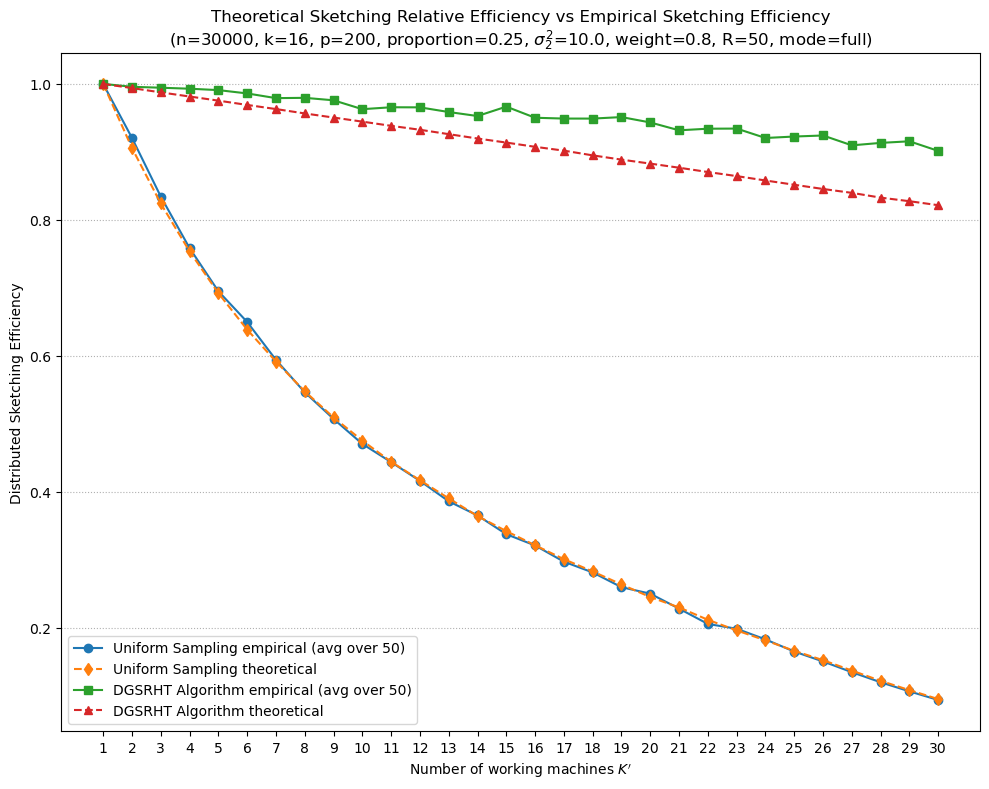
\includegraphics[width=0.85\textwidth]{full_result.png}
  \caption{Relative efficiency versus number of partition machines $K'$ under the fully heterogeneous GMM ($n=30{,}000$, $p=200$, $K=16$, $s=4$). Solid lines: empirical RE averaged over $R=50$ repetitions. Dashed lines: design-conditional theoretical RE from \eqref{eq:2.4}. DGSRHT (green/red) maintains RE near $1.0$ across all $K'$; uniform sampling (blue/orange) decays sharply as $K'$ grows.}
  \label{fig:re-full}
\end{figure}

\subsection{Discussion of experimental limitations}

The experiment above fixes one $(n,p)$ pair and one GMM configuration. Corollary~\ref{corollary:main} is an asymptotic statement requiring $\ln n = o(p)$ and $p\ln p = o(n)$; the chosen $(n,p)=(30{,}000,200)$ satisfies these conditions comfortably ($\ln n\approx 10.3 \ll 200$ and $p\ln p\approx 1{,}060 \ll 30{,}000$). As noted in Section~4.2, when $p$ grows linearly with $n$ the theoretical bound \eqref{eq:4.6} no longer guarantees convergence, and we expect the DGSRHT advantage to diminish in that regime.

\section{Discussion}
We would further focus on the proof of similar main result of Corollary~\ref{corollary:main} in the future work, and consider the case that $p$ is comparable to $n$ in the case that $p = c_1 n$ for any constant $c_1$. This is the case $p$ could also tends to infinity when $n$ is tending to infinity with the same level of infinite large. And we would try to use the method of integrated randomized matrix theory as a whole to prove it.

Our current result is conditioned on the distribution of Gaussian Mixture Model (GMM), which is a specific distribtuion and is not a common distribution, this result of merits of Randomzied Hadamard Transform (RHT) should be applied to more general settings of distributions. So we would further explore more general distribtions for RHT Sampling. 
\printbibliography %Prints bibliography
\end{document}